\documentclass[a4paper,10pt]{scrbook}
\usepackage{hyperref}

\usepackage{mathematix}
\usepackage[margin=1in,right=1in]{geometry}
\usepackage{lipsum}
\usepackage{enumerate}

\usepackage{caption}
\captionsetup{font=footnotesize,labelfont=bf}

\usepackage{natbib}
\usepackage{bibentry}
\nobibliography*

\renewcommand{\cov}{\operatorname{cov}}


\hypersetup{
    bookmarks=true,         % show bookmarks bar?
    unicode=false,          % non-Latin characters in Acrobat’s bookmarks
    pdftoolbar=true,        % show Acrobat’s toolbar?
    pdfmenubar=true,        % show Acrobat’s menu?
    pdffitwindow=false,     % window fit to page when opened
    pdfstartview={FitH},    % fits the width of the page to the window
    pdftitle={Probability Theory Cookbook},    % title
    pdfauthor={Pantelis Sopasakis},     % author
    pdfsubject={},   % subject of the document
    pdfcreator={P. Sopasakis},   % creator of the document
    pdfproducer={P. Sopasakis}, % producer of the document
    pdfnewwindow=true,      % links in new PDF window
    colorlinks=true,       % false: boxed links; true: colored links
    linkcolor=red,          % color of internal links (change box color with linkbordercolor)
    citecolor=green,        % color of links to bibliography
    filecolor=magenta,      % color of file links
    urlcolor=cyan           % color of external links
}

\newcommand{\ce}[1]{\E\left[#1 {}\mid{} \HH \right]}

% Update \bibentry so that bibentries appear in blue
\let\oldbibentry\bibentry
\renewcommand{\bibentry}[1]{{\color{blue} \oldbibentry{#1}}}

\title{Probability Cookbook}
\author{Pantelis Sopasakis}
\begin{document}
\maketitle
\tableofcontents

\addchap{Abstract}
  This document is intended to serve as a collection of important results in general probability
  theory, stochastic processes, uncertainty quantification, risk measures and a lot more.
  It can be used for a quick brush up or as a quick reference or 
  cheat sheet for graduate students and researchers in the domain of mathematics and 
  engineering. 
  The readers may find a list of bibliographic references with comments at the end
  of this document. This is still work in progress, so several important results are 
  still missing
% \end{abstract}

\chapter{Probability Theory}
\section{General Probability Theory}

\subsection{Measurable and Probability spaces}

\begin{enumerate}
 \item ($\sigma$-algebra). Let $X$ be a nonempty set. A collection $\F$ of subsets of $X$
       is called a $\sigma$-algebra if (i) $X \in \F$, (i) $A^c\in\F$ whenever $A\in\F$,
       (ii) if $A_1,\ldots, A_n\in\F$, then $\bigcup_{i=1,\ldots,n}A_i\in\F$. The space $X$
       equipped with a $\sigma$-algebra $\F$ is called a \textit{measurable space}.
       
 \item (d-system) A collection $\mathcal{D}$ of subsets of $X$ is called a d-system or a Dynkin class if 
       (i) $X\in\mathcal{D}$,
       (ii) $A\setminus B\in\mathcal{D}$ whenever $A,B\in\mathcal{D}$ and $A\supseteq B$,
       (iii) $A\in\mathcal{D}$ whenever $A_n\in \mathcal{D}$ and $A_n \uparrow A$ (meaning, 
       $A_{k}\subseteq A_{k+1}$ and $\bigcup_{k\in\N}A_k=A$).
       
 \item (p-system). A collection of sets $\mathcal{P}$ in $X$ is called a p-system
       if $A\cap B\in \mathcal{P}$ whenever $A,B\in\mathcal{P}$.
       
 \item A collection of sets is a $\sigma$-algebra if and only if it is both a p- and a d-system.
 
 \item (Smallest $\sigma$-algebra). Let $\HH$ be a collection of sets in $X$. The smallest collection of sets
       which contains $\HH$ and is a $\sigma$-algebra exists and is denoted by $\sigma(\HH)$.
 
 \item (Monotone class theorem). If a d-system $\mathcal{D}$ contains a p-system $\mathcal{P}$, then is also contains $\sigma(\mathcal{P})$.
 
 \item \label{mps1311949}
       (Borel $\sigma$-algebra). On $\Re$, the $\sigma$-algebra $\sigma(\{(a,b); a<b\})$ is called the Borel $\sigma$-algebra on $\Re$
       which we denote by $\B_\Re$. For topological spaces $(X,\tau)$, the Borel $\sigma$-algebra is
       defined as $\B_X = \sigma(\tau)$, i.e., it is the smallest $\sigma$-algebra which contains
       all open sets. $\B_\Re$ is generated by:
       \begin{enumerate}[i.]
        \item The open intervals $(a,b)$
        \item The closed intervals $[a,b]$
        \item All sets of the form $[a,b)$ or $(a,b]$
        \item Open rays $(a,\infty)$ or $(-\infty,a)$
        \item Closed rays $[a,\infty)$ or $(-\infty,a]$
       \end{enumerate}            

 \item (Measure). A function $\mu: \F\to [0,+\infty]$ is called a measure if 
       for every sequence of disjoint sets $A_n$ from $\F$, $\mu(\bigcup_n A_n)= \sum_n \mu(A_n)$.

 \item \label{mps1311960}
      (Properties of measures). The following hold:
      \begin{enumerate}[i.]
       \item (Empty set is negligible). $\mu(\varnothing)=0$ [Indeed, $\mu(A) = \mu(A\cup \varnothing) = \mu(A) + \mu(\varnothing)$ for all $A\in\F$]
       \item (Monotonicity). $A\subseteq B$ implies $\mu(A) \leq \mu(B)$ [Indeed, $\mu(B) = \mu(A\cup (B\setminus A))$]
       \item (Boole's inequality). For all $A_n\in\F$, $\mu(\bigcup_n A_n) \leq \sum_n \mu(A_n)$
       \item (Sequential continuity). If $A_n\uparrow A$, then $\mu(A_n)\uparrow \mu(A)$.
      \end{enumerate}

 \item (Equality of measures). Let $\mu,\nu$ be two measures on a measurable space $(X,\F)$ and let $\G$ 
       be a p-system generating $\F$. If $\mu(A) = \nu(A)$ for all $A\in \G$, then $\mu(B) = \nu(B)$
       for all $B\in\F$. As presented in \#\ref{mps1311949} above, p-systems are often available and 
       have simple forms.
      
 \item (Completeness). A measure space $(X,\F,\mu)$ is called \textit{complete} if the following holds:
	\[
	    A \in \F, \mu(A)=0, B\subseteq A \Rightarrow B \in \F.
	\]
       Of course, by the monotonicity property in \#\ref{mps1311960}--iii, if $(X,\F,\mu)$ is a complete 
       measure space then $\mu(B) = 0$.
       
 \item (Completion). Let $(X,\F,\mu)$ be a measure space and define the set of \textit{negligible sets} of $\mu$ as 
       $Z_\mu = \{N \subseteq X: \exists N'\supseteq N, N'\in\F \text{ s.t. } \mu(N')=0\}$.
       Let $\F'$ be the $\sigma$-algebra generated by $\F\cup Z_\mu$. Then
       \begin{enumerate}[i.]
        \item Every $B\in\F'$ can be written as $B=A\cup N$ with $A\in\F$ and $N\in Z_\mu$
        \item Define $\mu'(A\cup N) = \mu(A)$; this is a measure on $(X,\F')$ which renders 
              the space $(X,\F',\mu')$ complete. 
       \end{enumerate}
 
 \item (Lebesgue measure on $\Re$ and $\Re^n$). It suffices to define the \textit{Lebesgue measure} on $(\Re,\B_\Re)$
       on the p-system $\{(a,b), a<b\}$; it is $\lambda((a,b))=b - a$. This extends to a measure on  $(\Re,\B_\Re)$.
       Likewise, the collection of $n$-dimensional rectangles $\{(a_1, b_1)\times\ldots \times (a_n, b_n)\}$ is a p-system
       which generates $\B_{\Re^n}$; the Lebesgue measure on $(\Re^n, \B_{\Re^n})$ is 
       $\lambda(\prod_{i=1}^n (a_i, b_i))=\prod_{i=1}^n (b_i-a_i)$.
 
 \item (Lebesgue measurable sets). The completion of the Lebesgue measure defines the class of Lebesgue-measurable
       sets. 
             
 \item (Negligible boundary). If a set $C\subseteq \Re^n$ has a boundary whose Lebesgue measure is $0$, then 
       $C$ is Lebesgue measurable.
       
 \item (Independent events). Let $E_1,E_2$ be two events from $\ofp$; we say that $E_1$ and $E_2$ are \textit{independent}
       if $\prob[E_1\cap E_2] = \prob[E_1]\prob[E_2]$.
       
 \item (Independent $\sigma$-algebras). We say that two $\sigma$-algebras $\F_1$ and $\F_2$ on $\Omega$ 
       are independent if for any $E_1\in \F_1$ and $E_2\in\F_2$, $E_1$ and $E_2$ are independent.
       Note that $E_1\cap E_2$ is a member of the $\sigma$ algebra $E_1 \wedge E_2$.
       
 \item (Atom). Let $(\Omega, \F, \mu)$ be a measure space. A set $A\in\F$ is called an atom if
       $\mu(A)>0$ and for every $B\subset A$ with $\mu(B)<\mu(A)$ it is $\mu(B)=0$.
       A space without atoms is called non-atomic%
	    \footnote{A special class of spaces with (only) atoms are the discrete probability spaces where
	              $\F$ is generated by a discrete --- often finite --- set of events. Several 
	              results in measure theory require that the space be non-atomic. However, we may
	              often prove these results for discrete or finite spaces.}.
\end{enumerate}

\subsection{Random variables}\label{sec:random_variables}
\begin{enumerate}

 \item (Measurable function). A function $f:(X,\F)\to (Y,\G)$ (between two measurable spaces) is 
       called \textit{measurable} if $f^{-1}(G) \in \F$ for all $G\in\G$ (i.e., if it inverts all 
       measurable sets to measurable ones).
       
 \item (Measurability test). Let $\F,\G$ be $\sigma$-algebras on the nonempty sets $X$ and $Y$. Let $\G'$ be 
       a p-system which generates $\G$. A function $f: (X,\F)\to (Y,\G)$ is measurable 
       if and only if $f^{-1}(G')\in \F$ for all $G'\in\G'$ (it suffices to check the 
       measurability condition on a p-system).
       
 \item ($\sigma$-algebra generated by $f$). Let $f:(X,\F)\to (Y,\G)$ (between two measurable spaces) be a measurable
       function. The set 
       \[
        \sigma(f) \dfn \{f^{-1}(B){}\mid{} B\in \G\},
       \]
       is a sub-$\sigma$-algebra of $\F$ and is called the $\sigma$-algebra generated by $f$.
 
 \item (Preservation of measurability). Let \(f,g:\Omega\to\Re\) be two measurable functions on \((\Omega, \F)\).
       Then, the functions \(h_1(x) = f(x) + g(x)\), \(h_2(x) = f(x) - g(x)\),
       \(h_3(x) = \max\{f(x), g(x)\}\), \(h_4(x) = \min(f(x), g(x))\),
       \(h_5(x) = f(x)g(x)\) are measurable. For all \(\alpha\in\Re\), \(h_6(x) = \alpha f(x)\) is measurable.
       
 \item (Measurability of supermum/infimum). Let \((f_n)_n\) be a sequence of real-valued measurable 
       functions. Then \(\sup_n f_n\) and \(\inf_n f_n\) are measurable.
       
 \item (Sub/sup-level sets) Let $f:(X,\F)\to \Re$. The following are equivalent:
      \begin{enumerate}[i.]
       \item $f$ is measurable,
       \item Its \textit{sub-level sets}, that is
       sets of the form $\lev_{\leq \alpha} f \dfn \{x\in X: f(x) \leq \alpha\}$ are measurable,
	\item Its \textit{sup-level sets},
       that is sets of the form $\lev_{ \geq \alpha} f \dfn \{x\in X: f(x) \geq \alpha \}$ are 
       measurable. 
      \end{enumerate}

       
 \item \label{rv220000}
       (Random variable).
       A real-valued random variable $X:\ofp \to (\Re, \B_\Re)$ is a measurable function $X$
       from a probability space $\ofp$ to $\Re$, equipped with the Borel $\sigma$-algebra, that is, 
       for every Borel set $B$, $X^{-1}(B)\in\F$.              
       
 \item \label{rv221030}
      Every nonnegative (real-valued) random variable $X$ on $(\Re_+, \B_{{\Re}_+})$ 
      is written as 
      \[
        X(\omega) = \int_0^{+\infty} 1_{X(\omega)\geq t}\,\d t.
      \]

 \item (Increasing functions).  Every increasing function $f:\Re\to\barre$ is Borel-measurable.
 
 \item (Semi-continuous functions). Every lower semi-continuous function $X:\Omega\to\Re$ (where $\Omega$ is assumed 
       to be equipped with a topology) is Borel-measurable. 
       
 \item (Push-forward measure)~[\ref{cite:cinlar2011}]. Given measurable spaces $(\mathcal{X},\F)$ and $(\mathcal{Y}, \mathcal{G})$, 
 a measurable mapping $f: X \to Y$ and a (probability) measure $\mu$ on $(\mathcal{X},\F)$, the \textit{push-forward} of $\mu$
 is defined to be a measure $f∗(\mu)$ on $(\mathcal{Y}, \mathcal{G})$ given by
 \[
  (f_*\mu)(B) = \mu(f^{-1}(B)) = \mu(\{\omega\mid f(\omega)\in B\}),
 \]
 for $B\in\mathcal{G}$.
 \item (Change of variables). Let $F$ be a random variable on the probability space $\ofp$ and $F_*\prob$ 
 is the push-forward measure. random variable $X$ is integrable with respect to the push-forward measure $F_*\prob$
 if and only if $X\circ F$ is $\prob$-integrable. Then, the integrals coincide
 \[
  \int X \d(F_*\prob) = \int (X\circ F) \d \prob.
 \]
 \item (Measures from random variables). Let $X$ be a random variable on $\ofp$. 
       We may use $X$ to define the following measure
       \[
        \nu(A) = \int_A X\d \prob,
       \]
       defined for $A\in\F$. This is a positive measure which for short we denote as $\nu=X\prob$
       and it satisfies:
       \[
        \int_A Y\d \nu = \int_A XY\d \prob,
       \]
       for all random variables $Y$.
       
 \item (Compositions). Let $f:(X,\F_X)\to (Y, \F_Y)$ and $g:(Y,\F_Y)\to (Z,\F_Z)$ be two measurable functions. 
       Then, the function $h:(X,\F_X)\ni x\mapsto h(x) \dfn f(g(x)) \in (Z,\F_Z)$ is measurable. 
       
 \item (Simple function; definition). A simple function is one of the form
	\[
	 f(x) = \sum_{k=1}^{n}\alpha_k 1_{A_k}(x),
	\]
	where $1_{A_k}$ is the characteristic function of a measurable set $A_k$, that is
	\[
	 1_{A_k} = \begin{cases}
	            1,&\text{if }x\in A_{k}\\
	            0,&\text{otherwise}
	           \end{cases}
	\]



 \item (Characterization of measurability). A function $f:(X,\F)\to\Re$ is $\F$-measurable if and only if 
       it is the point-wise limit of a sequence of simple functions. A function $f:(X,\F)\to\Re_+$ is 
       $\F$-measurable if and only if  it is the point-wise limit of an increasing sequence of simple functions. 
       
 \item (Continuity and measurability). Every continuous function $f:(X,\F)\to\barre$ is Borel-measurable. 
  
 \item (Monotone class of functions). Let $M$ be a collection of functions $f:(X,\F)\to\barre$; let $M_+$
       be all positive functions in $M$ and $M_b$ all bounded functions in $M$. We say that $M$ is a \textit{monotone class}
       of functions if (i) $1\in M$, (ii) if $f,g\in M_b$ and $a,b\in \Re$, then $af+bg\in M$ and (iii)
       if $(f_n)_n\subseteq M_+$ and $f_n \uparrow f$, then $f\in M$.
       
 \item (Monotone class theorem for functions). Let $M$ be a monotone class of functions on $(X,\F)$. Suppose 
       that $\F$ is generated by some p-system $\mathcal{C}$, $1_A \in M$ for all $A\in\mathcal{C}$.
       Then, $M$ includes all positive $\F$-measurable functions and all bounded $\F$-measurable functions. 
       
 \item (Simple function approximation theorem).       
        Let $X$ be an extended-real-valued Lebesgue-measurable function defined on a Lebesgue measurable set $E$. 
        Then there exists a sequence $\{\phi_k\}_{k\in\N}$ of simple functions%
	    \footnote{A simple function is a finite linear combination of indicator functions of measurable sets, that is, 
	              simple functions are written as $\phi(x)=\sum_{i=1}^{n}\alpha_i 1_{A_i}(x)$. }
	 on $E$ such that
	\begin{enumerate}[i.]
	 \item $\phi_k\to X$, point-wise on $E$
	 \item $|\phi_k| \leq |X|$ on $E$ for all $k\in\N$
	\end{enumerate}
       If $X\geq 0$ then there exists a sequence of point-wise increasing simple functions with these properties.
       
  \item (Simple function approximation trick).         
        Let $f$ be a real-valued measurable function, $f:\ofp\to(\Re,\mathcal{B}_\Re)$. Define
        \[
         \phi_k(x) = \begin{cases}
                   \frac{j-1}{2^k},   &\frac{j-1}{2^k}\leq f(x) < \frac{j}{2^k}\\
                   k,                 &f(x) \geq k 
                  \end{cases}
        \]
        Then,
        \begin{enumerate}[i.]
         \item The sets $\{x: f(x) \geq k\}$ and $\{x: \frac{j-1}{2^k}\leq f(x) < \frac{j}{2^k}\}$ are measurable because $f$ is measurable
         \item $\phi_k$ are measurable for all $k\in\N$
         \item $\phi_k(x) \leq \phi_{k+1}(x)$ for all $k\in\N$ and for all $x\in\Omega$
         \item Let $E\subseteq \Omega$ so that $\sup_{x\in E}f(x) \leq M$. Then $\sup_{x\in\Omega}|f(x) - \phi_k(x)|\leq \nicefrac{1}{2^k}$ for all $k\geq M$
        \end{enumerate}

\end{enumerate}

\subsection{Limits}
\subsubsection{Limits of sequences of events}
\begin{enumerate}
 \item (Nested sequences and probabilities). Let $(E_n)_n$ be a non-increasing sequence of events ($E_n\supseteq E_{n+1}$ for all $n\in\N$). 
       Then $\lim_n \prob[E_n]$ exists and 
       \[
        \prob\left[\bigcap_n E_n\right] = \lim_n \prob[E_n].
       \]
       If $(E_n)_n$ is a nondecreasing sequence ($E_n \subseteq E_{n+1}$ for all $n\in\N$), then
       \[
        \prob\left[\bigcup_n E_n\right] = \lim_n \prob[E_n].
       \]


 \item (Limits inferior). For a sequence of events $E_n$, the \textit{limit inferior} of $(E_n)_n$
       is denoted by $\liminf_n E_n$ and is defined as 
       \[
        \liminf_n E_n = \bigcup_{n\in \N}\bigcap_{m\geq n}E_n = \{x:\ x\in E_n\ \text{for all but finitely many } n\in \N\}.
       \]
 \item (Limit superior). The \textit{limit superior} of $(E_n)_n$, $\limsup_n E_n$, is
       \[
        \limsup_n E_n = \bigcap_{n\in \N}\bigcup_{m\geq n}E_n = \{x:\ x\in E_n\ \text{infinitely often} \}.
       \]
 \item (Limits of complements). The limit (super/inferior) of a sequence of complements is the complement of the limit
	\begin{align*}
	 \liminf_n E_n^c &= (\limsup_n E_n)^c,\\
	 \limsup_n E_n^c &= (\liminf_n E_n)^c.
	\end{align*}

 \item (Relationship between limits). It is
       \[
        \liminf_n E_n \subseteq \limsup_n E_n.
       \]
 \item (Probabilities of $\liminf E_n$ and $\limsup E_n$). The sets $\liminf_n E_n$ and $\limsup_n E_n$ are measurable and 
 \[
  \prob[\liminf_n E_n] \leq \liminf_n \prob[E_n] \leq \limsup_n \prob[E_n] \leq \prob[\limsup_n E_n].
 \]
 
 \item (A result reminiscent of Baire's category theorem). Let $(E_n)_n$ be a sequence of almost sure events. Then
       $\prob[\cap_n E_n] = 1$.

 \item (Borel-Cantelli lemma). Let $(E_n)_n$ be a sequence of events over $\ofp$. The following hold
 \begin{enumerate}[i.]
  \item If $\sum_{n=1}^{\infty}\prob[E_n]<\infty$, then $\prob[\limsup_n E_n] = 0$
  \item If $(E_n)_n$ are independent events such that $\sum_{n=1}^{\infty}\prob[E_n]=\infty$, then
        $\prob[\limsup_n E_n] = 1$.
 \end{enumerate}
 
 \item (Corollary: Borel 0-1 law). If $(E_n)_n$ is a sequence of independent events, 
       then $\prob[\limsup_n E_n]\in\{0,1\}$ (according to the summability of $(\prob[E_n])_n$).

 \item (Kochen-Stoone lemma). Let $(E_n)_n$ be a sequence of events. Then,
 \[
  \prob[\limsup_n E_n] \geq \limsup_n \frac{\left(\sum_{k=1}^n \prob[A_k]\right)^2}{\sum_{k=1}^{n}\sum_{j=1}^{n}\prob[A_k\cap A_j]}
 \]
 
 \item (Corollary of Kochen-Stoone's lemma). If for $i\neq j$, $E_i$ and $E_j$ are either independent 
       or $\prob[E_i\cap E_j] \leq \prob[E_i]\prob[E_j]$ and $\sum_{n=1}^{\infty}\prob[E_n]=\infty$,
       then $\prob[\limsup_n E_n] = 1$.

\end{enumerate}



\subsubsection{Limits of sequences of random variables}
\begin{enumerate}
 \item (Lebesgue's monotone convergence theorem). Let $(f_n)_n$ be an increasing sequence of 
       nonnegative Borel functions and let $f \dfn \lim_n f_n$ (in the sense $f_n\to f$ point-wise a.e.). 
       Then $\E[f_n] \uparrow \E[f]$.
      
 \item 	(Lebesgue's Dominated Convergence Theorem). Let $X_n$ be real-valued RVs over $\ofp$. 
	Suppose that $X_n$ converges point-wise to $X$ and is \textit{dominated} by a 
	$Y\in\mathcal{L}_1\ofp$, that is $|X_n|\leq Y$ $\prob$-a.s for all $n\in\N$. 
	Then, $X\in\mathcal{L}_1\ofp$
	and
	\[
	 \lim_n \E[|X_n-X|] = 0,
	\]
        which implies
        \[
         \lim_n \E[X_n] = \E[X].
        \]

 \item (Dominated convergence in $\mathcal{L}^p$).
       For $p\in[1,\infty)$ and a sequence of random variables $X_k:\ofp\to\barre$,
       assume that $X_k\to X$ almost everywhere ($X(\omega)=\lim_k X_k(\omega)$ $\prob$-a.e.)
       and there is $Y\in\mathcal{L}^p\ofp$ so that $X_k\leq Y$. Then, 
       \begin{enumerate}[i.]
        \item $X_k\in\mathcal{L}^p\ofp$ for all $k\in\N$,
        \item $X\in\mathcal{L}^p\ofp$ 
        \item $X_k\to X$ in $\mathcal{L}^p\ofp$, that is $\lim_k \|X_k-X\|_p = 0$.
       \end{enumerate}

 \item (Consequence of the dominated convergence theorem)~[\ref{cite:DWalnut2011}]. 
       Let $\{E_k\}_{k=1}^{\infty}$ be a collection of disjoint events and let $E=\bigcup_{k}E_k$.
       Then,
       \[
        \int_E f = \sum_{k=1}^{\infty} \int_{E_k} f.
       \]

 \item  (Bounded convergence). If $X_k \to X$ almost surely and $\sup_k |X_k| \leq b$
        for some constant $b>0$, then $\E[X_k]\to \E[X]$ and $\E[|X|] \leq b$.
       
 \item 	(Fatou's lemma). Let $X_n\geq 0$ be a sequence of random variables. 
	Then, 
	\[
	\E[\liminf_n X_n] \leq  \liminf_n \E[X_n].
	\]
 \item 	(Fatou's lemma with varying measures). For a sequence of nonnegative random variables $X_n\geq 0$ over $\ofp$,
	and a sequence of (probability) measures $\mu_n$ which converge strongly to a (probability)
	measure $\mu$ (that is, $\mu_n(A)\to\mu(A)$ for all $A\in\F$), we have
	\[
	 \E_\mu[\liminf_n X_n]\leq \liminf_n \E_{\mu_n}[ X_n]
	\]

 \item 	(Reverse Fatou's lemma). Let $X_n\geq 0$ be a sequence of nonnegative random variables over $\ofp$ and
	assume there is a $Y\in\mathcal{L}_1\ofp$ so that $X_n\leq Y$. Then
	\[ 
	 \limsup_n \E[X_n] \leq \E[\limsup_n X_n]
	\]
 \item (Integrable lower bound). 	
	Let $X_n$ be a sequence of random variables over $\ofp$. Suppose, there exists a
	$Y\geq 0$ such that $X_n\geq -Y$ for all $n\in\N$. Then,
	\[
	\E[\liminf_n X_n] \leq  \liminf_n \E[X_n].
	\]
 \item (Beppo Levi's Theorem).
	Let $X_k$ be a sequence of nonnegative random variables on $\ofp$ with $0 \leq X_1 \leq X_{2} \leq \ldots$. 
	Let $X(\omega) = \lim_{k\to\infty}X_k(\omega)$. Then $X$ is a random variable and 
	\[
	 \lim_{k\to\infty} \E[X_k] = \E[\lim_{k\to\infty} X_k].
	\]
 \item (Beppo Levi's Theorem for series).
       Let $X_k$ be a sequence of nonnegative integrable random variables on $\ofp$
       and let $Y_k = \sum_{j=0}^k X_k$. Assume that $\sum_{k=1}^{\infty} \E[Y_k]$ converges.
       Then $Y_k$ satisfies the conditions of the BL theorem and
       \[
        \sum_{k=1}^{\infty} \E[Y_k] = \E \left[\sum_{k=1}^{\infty}Y_k\right].
       \]

 \item (Uniform integrability -- definition)~[\ref{cite:KSigman2009}]. A collection $\{X_k\}_{k\in T}$ is said to be \textit{uniformly
        integrable} if $\sup_{t\in T}\E[|X_t| 1_{|X_t|>x}] \to 0$ as $x\to\infty$.
        
 \item (Constant absolutely integrable sequences as uniformly integrable)~[\ref{cite:KSigman2009}]. The sequence $\{Y\}_{t\in T}$
       with $\E[|Y|]<\infty$ is uniformly integrable.

 \item (Uniform boundedness in $\mathcal{L}^p$, $p>1$, implies uniform integrability).
       If $\{X_t\}_{t\in T}$ is uniformly bounded in $\mathcal{L}^p$, $p>1$ (that is, 
       $\E[|X_k|^p] < c$ for some $c>0$), then it is uniformly integrable.
       
 \item (Convergence under uniform integrability)~[\ref{cite:KSigman2009}]. If $X_k \to X$ a.s. and $\{X_k\}_k$ is uniformly 
       integrable then
       \begin{enumerate}[i.]
         \item $\E[X]< \infty$
         \item $\E[X_k] \to \E[X]$        
        \item $\E|X_k-X|\to 0$
       \end{enumerate}

\end{enumerate}


\subsection{The Radon-Nikodym Theorem}
\begin{enumerate}
 \item (Absolute continuity).
       Let $(\mathcal{X}, \mathscr{G})$ be a measurable space and $\mu$ and $\nu$ two measures on it.
       We say that $\nu$ is \textit{absolutely continuous} with respect to $\mu$ if
       for all $A\in\mathscr{G}$, $\nu(A)=0$ whenever $\mu(A)=0$. We denote this by $\nu\ll\mu$.
 \item (Radon-Nikodym). Let $(\mathcal{X}, \mathscr{G})$ be a measurable space, let $\nu$ be a \textit{$\sigma$-finite}
       measure on $(\mathcal{X}, \mathscr{G})$ which is {absolutely continuous} with respect 
       to a measure $\mu$ on $(\mathcal{X}, \mathscr{G})$. Then, there is a measurable function $f:\mathcal{X}\to[0,\infty)$
       such that for all $A\in \mathcal{G}$
       \[
        \nu(A) = \int_A f \d \mu.
       \]
      This function is denoted by $f=\frac{\d\nu}{\d \mu}$.
 \item (Linearity). Let $\nu$, $\mu$ and $\lambda$ be $\sigma$-finite measures on $(\mathcal{X}, \mathscr{G})$ and $\nu\ll\lambda$, $\mu\ll\lambda$.
       Then
       \[
        \frac{\d(\nu+\mu)}{\d \lambda} = \frac{\d \nu}{\d \lambda} + \frac{\d \mu}{\d \lambda},\ \lambda\text{-a.e.}
       \]
 \item (Chain rule). If $\nu\ll\mu\ll\lambda$,
 \[
  \frac{\d\nu}{\d\lambda} = \frac{\d\nu}{\d\mu} \frac{\d\mu}{\d\lambda},\ \lambda\text{-a.e.} 
 \]
 \item (Inverse). If $\nu\ll\mu$ and $\mu\ll\nu$, then
 \[
  \frac{\d \mu}{\d \nu} = \left( \frac{\d \nu}{\d \mu}\right)^{-1},\ \nu\text{-a.e.}
 \]
 \item (Change of measure).
 If $\mu\ll\lambda$ and $g$ is a $\mu$-integrable function, then
 \[
  \int_{\mathcal{X}} g \d \mu = \int_{\mathcal{X}} g \frac{\d \mu}{\d \lambda}\d \lambda.
 \]
 \item (Change of variables in integration). This was addressed using the push-forward. 
 \[
  \E[g(X)] = \int g\circ X\d\prob = \int_\Re g \,\d(X_*\prob).
 \]
 If the measure $\d(X_*\prob)$ is absolutely continuous with respect to the Lebesgue 
 measure $\mu$ (on $(\Re, \B_\Re)$, then, the Radon-Nikodym derivative $f_X\dfn \frac{\d(X_*\prob)}{\d \mu}$,
 where $f_X:\Re\to\Re$ exists. Then
 \[
  \E[g(X)] = \int_\Re g\, \d(X_*\prob) = \int_\Re g f_X\, \d\mu = \int_\Re g(\tau)f_X(\tau)\,\d \tau.
 \]
 This is known as the \textit{law of the unconscious statistician} (LotUS).

\end{enumerate}




\subsection{Probability distribution}
\begin{enumerate} 
 
 \item (Probability distribution). Let $X:\ofp \to (Y, \G)$ be a random variable. The measure
 \[
  F_X(A) = \prob[X\in A] = \prob[\{\omega\in\Omega\mid X(\omega) \in A\}] = \prob[X^{-1}A] = (X_*\prob)(A),
 \]
 is called the \textit{probability distribution} of $X$ and it is a measure . Note that for all $A\in\G$, $X^{-1}A\in\F$
 since $X$ is measurable. 
 \item \label{rv221088}
 (Probability distribution of real-valued random variables).
 The \textit{probability distribution} or \textit{cumulative distribution function} of a random variable $X$ on a space
 $\mathcal{L}^p\ofp$ is $F_X(x) = \prob[X\leq x]$ for $x\in\Re$. The inverse cumulative
 distribution of $X$ is $F_X^{-1}(p)$ for $p\in[0,1]$ is defined as 
 $F_X^{-1}=\inf\{x\in\Re: F_X(x) \geq p\}$. 
 
 \item (Push-forward).
 \label{rv221089}
 The probability distribution of a random variable $X$ with values in $(\mathcal{X},\mathscr{G})$,
 is the push-forward measure $X_*\prob$ on $(\mathcal{X},\mathscr{G})$ which is 
 a probability measure on $(\mathcal{X},\mathscr{G})$ with $X_*\prob = \prob X^{-1}$.
 
 
 \item 
 \label{rv221137}
 We associate with $F_X:\Re\to[0,1]$ the measure $\mu$ which is defined on 
 the $p$-system $\{(-\infty,x]\}_{x\in\Re}$ as $\mu((-\infty, x]) = F_X(x)$.
 \item
 \label{rv231132}
 Properties of the cumulative and the inverse cumulative distributions. The notation
 $X\sim Y$ means that $X$ and $Y$ have the same cumulative distribution, that is 
 $F_X = F_Y$.
    \begin{enumerate}[i.]
      \item If $Y\sim U[0,1]$, then $F_X^{-1}(Y) \sim X$.
      \item $F_X$ is c\`adl\`ag
      \item $x_1<x_2 \Rightarrow F_X(x_1) \leq F_X(x_2)$
      \item $\prob[X>x] = 1 - F_X(x)$
      \item $\prob[\{x_1 < X \leq x_2\}] = F_X(x_2) - F_X(x_1)$
      \item $\lim_{x\to-\infty}F_X(x) = 0$, $\lim_{x\to\infty}F_X(x) = 1$
      \item $F_X^{-1}(F_X(x)) \leq x$
      \item $F_X(F_X^{-1}(p)) \geq p$
      \item $F_X^{-1}(p) \leq x \Leftrightarrow p \leq F_X(x)$
    \end{enumerate}
\end{enumerate}

\subsection{Probability density function}
\begin{enumerate}
 \item (Definition).
    The probability density function $f_X$ of a random variable $X:\ofp\to (\mathcal{X},\mathscr{G})$
    with respect to a measure $\mu$ on $(\mathcal{X},\mathscr{G})$ is the Radon-Nikodym derivative
    \[
     f_X = \frac{\d (X_*\prob)}{\d \mu},
    \]
    which exists provided that $X_*\prob \ll \mu$, and $f_X$ is measurable and $\mu$-integrable. Then,
    \begin{align*}
     \prob[X\in A] = \int_{X^{-1}A}\d \prob
                   = \int_{\Omega} 1_{X^{-1}A}\d\prob
                   = \int_{\Omega} (1_{A}\circ X)\d\prob
                   = \int_{A}\d(X_*\prob)
                   = \int_A f_X \d \mu.
    \end{align*}
  \item (Probability distribution).
	If $X$ is a real-valued random variable and its range ($\Re$) is taken with the 
        Borel $\sigma$-algebra, then 
        \begin{align*}
         \prob[X\leq x] = \int_{(-\infty, x]}X\d \prob
         = \int_{\{\omega\in\Omega: X(\omega) \leq x\}}\d \prob
         = \int_{-\infty}^x f_X\d \mu
        \end{align*}
        Note that the first integral is written with a slight abuse of notation as the 
        integration with respect to $\prob$ is carried out over the set $\{\omega\in\Omega: X(\omega) \leq x\}$;
        The first integral can be understood as shorthand notation for the second integral.
  \item (Expectation).
	Let a real-valued random variable $X$ have probability density $f_X$. Let $\iota$
	be the identity function $\iota:x\mapsto x$ on $\Omega$. Then
        \[
         \E[X] = \int_\Omega X\d\prob 
               = \int_\Omega (\iota\circ X)\d\prob 
               = \int_\Re \iota\d(X_*\prob)
               = \int_\Re \iota(x) f_X(x) \d\mu
               = \int_\Re x f_X(x) \d x.
        \]
  \item (Distribution of transformation). Let $g:\Re\to\Re$ be a strictly increasing function. 
         Let $X$ be a real-valued random variable with probability density function $f_X$ 
         and let $Y(\omega) = g(X(\omega))$ be another random variable. Then
  \begin{align*}
   F_Y(y) &= F_X(g^{-1}(y)),\\
   f_Y(y) &= f_X(g^{-1}(y))\frac{\partial g^{-1}(y)}{\partial y}.
  \end{align*}
  
  \item (Expectation of transformation). Let $X$ be a real-valued random variable on \(\ofp\) with 
  probability density function \(f_X\) and let $Y(\omega) = g(X(\omega))$  
  be another random variable. Then
  \[
   \E[Y] = \int_{-\infty}^{\infty} f_X(\tau) g(\tau) \d \tau.
  \]
  If $\Omega=\{\omega_i\}_{i=1}^{n}$, $\F=2^\Omega$ and $\prob[\{\omega\}_i] = p_i$, then
  \[
   \E[Y] = \sum_{i=1}^{n}p_i g(X(\omega_i)).
  \]
  See also: law of the unconscious statistician.


\end{enumerate}

\subsection{Decomposition of measures}
Does a density function always exist? The answer is negative, but Lebesgue's decomposition 
theorem offers some further insight. 
\begin{enumerate}
 \item (Singular measures). Let $(\Omega, \F)$ be a measurable space and $\mu$, $\nu$
       be two measures defined thereon. These are called \textit{singular} if there are 
       $A,B\in\F$ so that
       \begin{enumerate}[i.]
        \item $A\cup B=\Omega$, 
        \item $A\cap B=\varnothing$,
        \item $\mu(B')=0$ for all $B'\in\F$ with $B'\subseteq B$,
        \item $\nu(A')=0$ for all $A'\in\F$ with $A'\subseteq A$.
       \end{enumerate}
 \item (Discrete measure on $\Re$). A measure $\mu$ on $\Re$ equipped with the Lebesgue $\sigma$-algebra,
       is said to be discrete if there is a (possibly finite) sequence of elements $\{s_k\}_{k\in\N}$,
       so that 
       \[
        \mu(\Re\setminus \bigcup_{k\in\N} \{s_k\}) = 0.
       \]
 \item (Lebesgue's decomposition Theorem). For every two $\sigma$-finite signed measures $\mu$ and $\nu$
       on a measurable space $(\Omega, \F)$, there exist two $\sigma$-finite signed measures $\nu_0$ and $\nu_1$ 
       on $(\Omega, \F)$ such that
       \begin{enumerate}[i.]
        \item $\nu = \nu_0 + \nu_1$
        \item $\nu_0\ll \mu$
        \item $\nu_1 {}\bot{} \mu$
       \end{enumerate}
       and $\nu_0$ and $\nu_1$ are uniquely determined by $\nu$ and $\mu$.
\item (Lebesgue's decomposition Theorem --- Corollary).
      Consider the space $(\Re,\B_\Re)$ and let $\mu$ be the Lebesgue measure. Any probability measure $\nu$
      on this space can be written as
      \[
       \nu = \nu_{\text{ac}} + \nu_{\text{sc}} + \nu_{\text{d}},
      \]
      where $\nu_{\text{ac}} \ll \mu$ (which is easily understood via the 
      Radon-Nikodym Theorem), $\nu_{\text{sc}}$ is singular continuous (wrt $\mu$) and $\nu_{\text{d}}$
      is a discrete measure.
             
\end{enumerate}

\subsection{$\mathcal{L}^p$ spaces}
\begin{enumerate}
 \item ($p$-norm). Let $X$ be a real-valued random variable on $\ofp$. For $p\in[1,\infty)$ define the $p$-norm of $X$ as 
       \[
        \|X\|_p = \E[|X|^p]^{1/p}.
       \]
 \item ($\mathfrak{L}^p$ spaces). Define $\mathfrak{L}^p\ofp=\{X:\Omega\to\Re,\text{ measurable}, 
       \|X\|_p<\infty\}$ and equip this space with the addition and scalar multiplication 
       operations $(X+Y)(\omega) = X(\omega) + Y(\omega)$ and $(\alpha X)(\omega) = \alpha X(\omega)$.
       This becomes a semi-normed space%
	  \footnote{$\|X\|=0$ does not imply that $X=0$, but instead 
		    that $X=0$ almost surely. However, $\|\cdot\|_p$ is absolutely 
		    homogeneous, sub-additive and nonnegative}.%
 \item ($\mathcal{L}^p$ spaces). Define $\mathcal{N}\ofp = \{X:\Omega\to\Re,
       \text{ measurable}, X=0 \text{ a.s.}\}$; this is the kernel of $\|\cdot\|_p$. 
       Then, define $\mathcal{L}^p\ofp = \mathfrak{L}^p\ofp / \mathcal{N}$.
       This is a normed space where for $X\in\mathfrak{L}^p\ofp$ and $[X]=X+\mathcal{N}\in\mathcal{L}^p\ofp$
       we have $\|[X]\|_p \dfn \|X\|_p$.
 \item ($\infty$-norm, $\mathfrak{L}_\infty$ and $\mathcal{L}_\infty$). The infinity norm is defined as 
	\[
	 \|X\|_\infty = \esssup |X| = \inf\{\lambda \in \Re: \prob[|X|> \lambda] = 0\},
	\]
	or equivalently 
	\[
	 \|X\|_\infty = \inf \{\lambda \in \Re: |X|\leq \lambda,\, \prob\text{-a.s.}\}.
	\]
	The spaces $\mathfrak{L}_\infty\ofp$ and $\mathcal{L}_\infty\ofp$ are defined 
	similarly.
 \item ($\mathcal{L}_\infty\ofp$ as a limit). If there is a $p'\in [1,\infty)$ such 
       that $X\in\mathcal{L}_\infty\cap \mathcal{L}_{p'}$, then
       \[
        \|X\|_\infty = \lim_{p\to\infty}\|X\|_p.
       \]

 \item ($\mathcal{L}_2$ is a Hilbert space). $\mathcal{L}^p\ofp$ is the only Hilbert 
       $\mathcal{L}^p$ space with inner product
       \[
        \<X,Y\> = \E[XY].
       \]


\end{enumerate}


\subsection{Product spaces}
\begin{enumerate}
 \item (Product $\sigma$-algebra). Let $\{X_a\}_{a\in A}$ be an indexed collection of nonempty sets; define 
       $X=\prod_{a\in A}X_a$ and $\pi_a: X = (x_a)_{a\in A} \mapsto x_a\in X_a$. Let $\F_a$ be a $\sigma$-algebra
       on $X_a$. We define the product $\sigma$-algebra as
       \[
        \bigotimes_{a\in A} \F_a \dfn \sigma\left( \{\pi_a^{-1}(E_a);a\in A, E_a\in \F_a\}\right)
       \]
       This is the smallest $\sigma$-algebra on the product space which renders all projections measurable
       (compare to the definition of the \textit{product topology} which is the smallest topology on 
       the product space which renders the projections \textit{continuous}).
       
 \item (Measurability of epigraphs). Let $f:(X,\F)\to\barre$ be a measurable proper function. Its epigraph, that is
       the set $\epi f \dfn \{(x,\alpha)\in X\times \Re {}\mid{} f(x) \leq \alpha\}$ and its hypo-graph, that is
       the set $\hyp f \dfn \{(x,\alpha) \in X\times \Re {}\mid{} f(x) \geq \alpha\}$ are measurable in the product
       measure space $(X\times \Re, \F\otimes \B_\Re)$.
       
 \item (Measurability of graph). The graph of a measurable function $f:(X,\F,\mu)\to\Re$ is a Lebesgue-measurable set 
       with Lebesgue measure zero.
       
 \item (Countable product of $\sigma$-algebras). If $A$ is countable, the product $\sigma$-algebra       
       is generated by the products of measurable sets $\{\prod_{a\in A}E_a; E_a\in \F_a\}$.
       
 \item (Product measures). Let $(\mathcal{X},\F,\mu)$ and $(\mathcal{Y},\mathcal{G},\nu)$ be two measure spaces.
       The product space $\mathcal{X}\times \mathcal{Y}$ becomes a measurable space with the $\sigma$-algebra 
       $\F\otimes \mathcal{G}$. Let $E_x\in\F$ and $E_y\in\mathcal{G}$; then $E_x\times E_y\in\F\otimes \mathcal{G}$.
       We define a measure $\mu\times\nu$ on $(\mathcal{X}\times \mathcal{Y}, \F\otimes\mathcal{G})$ with 
       \[
        (\mu\times \nu)(E_x\times E_y) = \mu(E_x) \nu(E_y).
       \]
       
 \item Let $E\in \F\otimes\mathcal{G}$ and define 
       $E_x = \{y\in \mathcal{Y}: (x,y)\in E\}$ and $E_y = \{x\in \mathcal{X}: (x,y)\in E\}$.
       Then, $E_x\in \F$ for all $x\in\mathcal{X}$, $E_y\in\mathcal{G}$ for all $y\in\mathcal{Y}$.
 \item Let $f:\mathcal{X}\times\mathcal{Y}\to \Re$ be an $\F\otimes \mathcal{G}$-measurable function.
       Then, $f(x,\cdot)$ is $\mathcal{G}$-measurable for all $x\in\mathcal{X}$ and 
       $f(\cdot, y)$ is $\F$-measurable for all $y\in\mathcal{Y}$.
 \item Let $(\mathcal{X},\F,\mu)$ and $(\mathcal{Y},\mathcal{G},\nu)$ be two $\sigma$-finite measure spaces.
       For $E\in\F\otimes\mathcal{G}$, the mappings $\mathcal{X}\ni x\mapsto \nu(E_x) \in \Re$ and 
       $\mathcal{Y}\ni y\mapsto \mu(E_y)$ are measurable and
       \[
        (\mu\times \nu)(E) = \int \nu(E_x)\d \mu(x) = \int \mu(E_y)\d \nu(x)
       \]
 \item (Tonelli's Theorem). Let $h:\mathcal{X}\times \mathcal{Y}\to[0,\infty]$ be an $\F\otimes\mathcal{G}$-measurable
       function. Let
       \[
        f(x) = \int_{\mathcal{Y}} h(x,y) \d\nu(y), \ g(y) = \int_{\mathcal{X}}h(x,y)\d\mu(x).
       \]
       Then, $f$ and $g$ are measurable and 
       \[
        \int_{\mathcal{X}}f\d\mu = \int_{\mathcal{Y}}g\d\nu = \int_{\mathcal{X}\times\mathcal{Y}}g\d(\mu\times \nu).
       \]
 \item (Fubini's Theorem). 
       Let $h:\mathcal{X}\times \mathcal{Y}\to \Re$ be an $\F\otimes\mathcal{G}$-measurable
       function and
       \[
        \int_{\mathcal{X}} \int_{\mathcal{Y}} h(x,y)\d\nu(y) \d\mu(x) < \infty.
       \]
       Then, $h\in\mathcal{L}_1(\mathcal{X}\times\mathcal{Y}, \F\otimes\mathcal{G}, \mu\times\nu)$ and
        \[
        \int_{\mathcal{X}} \int_{\mathcal{Y}} h(x,y)\d\nu(y) \d\mu(x) = 
        \int_{\mathcal{Y}} \int_{\mathcal{X}} h(x,y)\d\mu(x) \d\nu(y) = 
        \int_{\mathcal{X}\times\mathcal{Y}} h \d(\mu\times \nu)
       \]
       
 \item (Consequence of Fubini's theorem). Let $X$ be a nonnegative random variable. Let $E=\{(\omega, x): 0 \leq x\leq X(\omega)\}$.
       Then, $X(\omega) = \int_{0}^{\infty}1_{E}(\omega, x)\d x$.
       \begin{align*}
        \E[X] = \int_{\Omega}X\d\prob &= \int_{\Omega}\int_{0}^{\infty}1_{E}(\omega, x)\d x\d \prob\\
                                      &= \int_{0}^{\infty} \int_{\Omega} 1_{E}(\omega, x)\d \prob \d x\\
                                      &= \int_{0}^{\infty} \prob[X\geq x]\d x.
       \end{align*}

\end{enumerate}

\subsection{Transition Kernels}\label{sec:transition_kernel}
\begin{enumerate}
 \item (Definition). Let $(\mathcal{X},\F)$, $(\mathcal{Y},\G)$ be two measurable spaces and let $K:\G\times \mathcal{X}\to [0,1]$.
       $K$ is called a \textit{(probability) transition kernel} if
       \begin{enumerate}[i.]
        \item $f_B(x) \dfn K(B,x)$ is $\F$-measurable for every $B\in\G$,
        \item $\mu_x(B) \dfn K(B,x)$ is a measure on $(\mathcal{Y},\G)$ for every $x\in \mathcal{X}$.
       \end{enumerate}
 \item (Markov kernel). A kernel $K:\G\times \mathcal{X}\to [0,1]$ is called a \textit{Markov kernel} if 
       $K(\mathcal{Y}, x)=1$ for all $x\in\mathcal{X}$
 \item (Existence of transition kernels). Let $\mu$ be a finite measure on 
       $(\mathcal{X},\F)$ and $k:\mathcal{X}\times \mathcal{Y}\to\Re_+$
       be measurable in the product $\sigma$-algebra $\F\otimes \G$ and has the property $\int_{\mathcal{Y}} k(x,y)\nu(\d y)=1$. Then
       the mapping $K:\mathcal{X} \times \G \to [0,1]$ given by
       \[
        K(B,x) = \int_B k(x,y) \mu(\d y),
       \]
       is a probability transition kernel.
 \item (Measure on product space via a kernel). 
       Let $(\mathcal{X},\F)$, $(\mathcal{Y},\G)$ be two measurable spaces and let $K:\G\times\mathcal{X}\to [0,1]$
       be a transition kernel. For $A\in\F$ and $B\in\G$ define 
       \[
        \mu(A\times B) = \int_A K(B,x)\d\prob(x).
       \]
       This extends to a unique measure on the product space $(\mathcal{X}\times\mathcal{Y}, \F\otimes\G)$.
\end{enumerate}

\subsection{Law invariance}
\begin{enumerate}
 \item (Equality in distribution). 
      Let $X,Y$ be two real-valued random variables on $\ofp$.
      We say that $X$ and $Y$ are equal in distribution, and we denote $X\overset{\mathrm{d}}{\sim} Y$,
      if $X$ and $Y$ have equal probability distribution functions, that is $F_X(s) = F_Y(s)$ for all $s$.

 \item (Equal in distribution, nowhere equal). Let $\Omega = \{-1,1\}$, $\F=2^\Omega$, $\prob[\{\omega_i\}]=\frac{1}{2}$.
       Let $X(\omega) = \omega$ and $Y(\omega) = -X(\omega)$. These two variables have the same distribution, but 
       are nowhere equal.
 
 \item (Equal in distribution, almost nowhere equal). Take $X\sim \mathcal{N}(0,1)$ and $Y=-X$. These 
       two random variables are almost nowhere equal, but have the same distribution.
       
 \item The following are equivalent:
      \begin{enumerate}[i.]
       \item $X\overset{\mathrm{d}}{\sim} Y$
       \item $\E[e^{-rX}]=\E[e^{-rY}]$ for all $r>0$
       \item $\E[f(X)] = \E[f(Y)]$ for all bounded continuous functions
       \item $\E[f(X)] = \E[f(Y)]$ for all bounded Borel functions
       \item $\E[f(X)] = \E[f(Y)]$ for all positive Borel functions	
      \end{enumerate}

\end{enumerate}


\subsection{Expectation}
\begin{enumerate}  
\item (Definition)
 Let $\ofp$ be a probability space and $X$ be a random variable. Then, the expected value of 
 $X$ is denoted by $\E[X]$ and is defined as the Lebesgue integral
 \[
  \E[X] = \int_{\Omega} X\d \prob
 \]

\item 
 \label{gx1312}
 Because of item~\ref{rv221030} in Sec.~\ref{sec:random_variables}, for $X\geq 0$ nonnegative 
 \begin{align*}
  \E[X] &= \int_{0}^{+\infty} X \d \prob\\
        &= \int_{0}^{+\infty} \int_0^{+\infty} 1_{X\geq t}\d t \d \prob\\
        &= \int_{0}^{+\infty} \int_0^{+\infty} 1_{X\geq t} \d \prob \d t
 \end{align*}
 and we use the fact that 
 \[
  \int_{0}^{+\infty} 1_{X>t}\d \prob = \prob[X>t],
 \]
 so
 \[
  \E[X] = \int_0^\infty \prob[X>t]\d t.
 \]
 The function $S(t) = \prob[X>t] = 1-\prob[X\leq t]$ is called the \textit{survival function} 
 of $X$, or its \textit{tail distribution} or \textit{exceedance}.

 \item (Expectation in terms of PDF). Let \(X\) be a real-valued continuous random variable with PDF \(f_X\). 
       Then,
       \[
        \E[X] = \int_{-\infty}^{\infty} x f_X(x) \d x.
       \]
 \item (Expectation in terms of CDF). Let \(X\) be a real-valued random variable. Then,
 \[
  \E[X] = \int_{-\infty}^{\infty} x \d F(x).
 \]

 \item Let $\ofp$ be a probability space and $X$ a real-valued random variable thereon. Define 
 \[
  f(\tau) = \int_{\Omega}(X-\tau)^2\d\prob.
 \]
 Then $\tau = \E[X]$ minimizes $f$ and the minimum value is $\mathrm{Var}[X]$.
 \item Let $X$ be a real-valued random variable. Then,
 \[
  \sum_{n=1}^{\infty}\prob[|X|\geq n] \leq \E[|X|] \leq 1+ \sum_{n=1}^{\infty}\prob[|X|\geq n].
 \]
 It is $\E[|X|]<\infty$ if and only if the above series converges.
 \item If $X$ takes positive integer values, then
 \[
  \E[X] = \sum_{n=1}^{\infty}\prob[X\geq n]
 \]

 \item (Finite mean, infinite variance). There are several distributions with finite mean 
       and infinite variance --- a standard example is the \textit{Pareto distribution}.
       A random variable $X$ follows the Pareto distribution with parameters $x_m>0$ and $a$
       if it has support $[x_m,\infty)$ and probability distribution
       \[
        \prob[X\leq x] = \frac{ax_m^a}{x^{a+1}},
       \]
       for $x\geq x_m$. For $a\leq 1$, $X$ has infinite mean and variance. For $a>1$, its
       mean is $\E[X]=\frac{ax_m}{a-1}$ and infinite variance.
       
 \item (Absolutely bounded a.s. $\Leftrightarrow$ Bounded moments)~[\ref{cite:Ambrosio2013}].
	Let $X$ be a random variable on $\ofp$. The following are equivalent:
	\begin{enumerate}[i.]
	  \item $X$ is almost surely absolutely bounded (i.e., there is $M\geq 0$ such that $\prob[|X|\leq M]=1$)
	  \item $\E[|X|^k]\leq M^k$, for all $k\in \N_{\geq 1}$
	\end{enumerate}

 \item (A useful formula)~[\ref{cite:RLWolpert05}]. For $q>0$
 \[
  \E[|X|^q] = \int_0^\infty q x^{q-1} \prob[|X|>x]\d x.
 \]	

\end{enumerate}




\section{Conditioning}
\subsection{Conditional Expectation}
\begin{enumerate}
 \item (Conditional Expectation). Let $X$ be a random variable on $\ofp$ and $\HH\subseteq \F$.
       A \textit{conditional expectation} of $X$ given $\HH$ is an $\HH$-measurable 
       random variable, denoted as $\ce{X}$, with
       \[
        \int_H \ce{X} \d\prob = \int_H X\d\prob,
       \]
       which equivalently can be written as
       \[
        \E[X 1_H] = \E[\ce{X}1_H],
       \]
       for all $H\in\HH$.
 \item (Uniqueness). All versions of a conditional expectation, $\ce{X}$, differ only on a 
       set of measure zero%
       \footnote{R. Durrett, ``Probability: Theory and Examples,'' 2013, Available at: \url{https://services.math.duke.edu/~rtd/PTE/PTE4_1.pdf}}.
 \item (Equivalent definition). It is equivalent to define the conditional expectation of $X$, 
       conditioned by a $\sigma$-algebra $\HH$ as a random variable $\ce{X}$ with the property
       \[
        \E[X Z] = \E[\ce{X}Z],
       \]
       for all $\HH$-measurable random variables $Z$.
 \item (Best estimator). Assuming $\E[Y^2]<\infty$, the best estimator of $Y$ given $X$ is $\E[Y{}\mid{}X]$      
 \item (Radon-Nikodym definition). The conditional expectation as introduced above, is the Radon-Nikodym
       derivative
       \[
          \ce{X} = \frac{\d \mu^X_{\HH}}{\d \prob_{\HH}},
       \]
      where $\mu^X_{\HH}:\HH\to [0,\infty]$ is the measure induced by $X$
      restricted on $\HH$, that is $\mu^X_{\HH}:H\mapsto \int_H X\d\prob$.
      This is absolutely continuous with respect to $\prob$. The measure $\prob_{\HH}$
      is the restriction of $\prob$ on $\HH$. 
      
 \item (Conditional expectation wrt random variable). Let $X,Y$ be random variables on $\ofp$.
       The conditional expectation of $X$ given $Y$ is $\E[X\mid Y]\dfn \E[X\mid \sigma(Y)]$,
       where $\sigma(Y)$ is the $\sigma$-algebra generated by $Y$, that is 
       $\sigma(Y) = Y^{-1}(\F) = \{Y^{-1}(B); B\in\F\}$.
       
 \item (Conditional expectation using the push-forward $Y_*\prob$). 
       Let $X$ be an integrable random variable on $\ofp$. Then, there is a $Y_*\prob$-unique 
       random variable $\E[X\mid Y]$
       \[
        \int_{Y^{-1}(B)} X\d \prob = \int_B \E[X{}\mid{}Y]\d(Y_*\prob).
       \]

 \item (Conditioning by an event). The conditional expectation $\E[X\mid H]$, conditioned
       by an event $H\in\F$ is given by
       \[
        \E[X\mid H] = \frac{1}{\prob[H]}\int_H X\d\prob = \frac{1}{\prob[H]}\E[X1_H].
       \]

 \item (Properties of conditional expectations). 
       The conditional expectation has the following properties:
       \begin{enumerate}[i.]
	\item \label{tp01} (Monotonicity). $X\leq Y \Rightarrow \ce{X} \leq \ce{Y}$
	\item (Positivity).  $X\geq 0 \Rightarrow \ce{X} \geq 0$ [Set $Y=0$ in~\ref{tp01}]. 
	\item (Linearity). For $a,b\in\Re$, $\ce{aX+bY}=a\ce{X} + b \ce{Y}$
	\item (Monotone convergence). $X_n\geq 0$, $X_n \uparrow X$ implies $\ce{X_n}\uparrow \ce{X}$
	\item (Fatou's lemma). For $X_n\geq 0$, $\ce{\liminf_n X_n}\leq \liminf_n \ce{X_n}$
	\item (Reverse Fatou's lemma). 
	\item (Dominated convergence theorem). $X_n\to X$ (point-wise) and $|X_n|\leq Y$ $\prob$-a.s. where $Y$ is
	      integrable. Then, $\ce{X}$ is integrable and 
	      \[
	       \ce{X_n} \to \ce{X}.
	      \]
        \item (Jensen's inequality). Let $X\in\mathcal{L}_1\ofp$, $f:\Re\to\Re$ convex. Then
	      \[
	      f(\ce{X})\leq \ce{f(X)}.
	      \]
        \item (Law of total expectation). For any $\sigma$-algebra $\HH \subseteq \F$,
	      \[
	       \E[\ce{X}] = \E[X].
	      \]
        \item (Tower property). For two $\sigma$-algebras $\HH_1$ and $\HH_2$ with $\HH_1\subseteq \HH_2$,	      
	      \[
	       \E[\E[X {}\mid{} \HH_1] {}\mid{} \HH_2] = \E[\E[X {}\mid{} \HH_2] {}\mid{} \HH_1] = \E[X {}\mid{} \HH_1].
	      \]
        \item (Tower property with $X$ being $\HH_i$-measurable). Let $\HH_1\subseteq \HH_2$ be two $\sigma$-algebras. 
	      If $X$ is $\HH_1$-measurable, then it is also $\HH_2$-measurable.
	    

        \item If $X$ is $\HH$-measurable then
	      \[
	       \ce{X} = X.
	      \]

       \end{enumerate}
       %
       %
       % CHECK A LOT MORE INTERESTING RESULTS IN: ASH DOLEANS
       %
\end{enumerate}


\subsection{Conditional Probability}
\begin{enumerate}
 \item (Conditional probability). Let $\ofp$ be a probability space and $\HH$ be a sub-$\sigma$-algebra
       of $\F$. We define $\prob_{\HH}$ as an operator so that for all $H\in\HH$
       \[
        \prob_{\HH}[H] = \E_{\F}1_{H}.
       \]
 \item (Conditional probability given an event). For $E,H\in\F$, $\prob[E\cap H] = \prob[H]\prob_{H}[E]$. This is
       uniquely defined provided that $\prob[H]>0$.
\end{enumerate}

\subsection{Construction of probability spaces}
\begin{enumerate}
 \item (Inonescu-Tulcea's Theorem). 
 \item (Kolmogorov's Extension Theorem). Let \(T\) denote a time interval, \(k\in\N\) and let 
       \(\nu_{t_1,\ldots, t_k}\) be probability measures on \(\Re^{nk}\) such that 
       \begin{enumerate}
        \item For all permutations \(\pi\) on \(\{1,\ldots, k\}\) it holds that 
        \[
	      \nu_{\pi(t_1),\ldots, \pi(t_k)}(F_1\times\cdots\times F_k)
	      {}={} 
	      \nu_{t_1,\ldots, t_k}(F_{\pi^{-1}(1)}\times \cdots \times F_{\pi^{-1}(k)}),
	\]
	\item For all \(m\in\N\) the following holds 
	\[
		\nu_{t_1,\ldots, t_k}(F_1\times\cdots\times F_k)
		=
		\nu_{t_1,\ldots, t_k,t_{k+1},\ldots, t_{k+1}}(F_1\times\cdots\times F_k\times \Re^n\times \cdots \times \Re^n).
	\]
       \end{enumerate}
      Then, there exists a probability space \(\ofp\) and a stochastic process \((X_t)_t\) on \(\Omega\) such that 
      \[
       \nu_{t_1,\ldots, t_k}(F_1\times\cdots\times F_k) = \prob[X_{t_1}\in F_1, \ldots, X_{t_k}\in F_k],
      \]
      for all Borel sets \(F_i\), \(i=1,\ldots, k\).
      

\end{enumerate}



\section{Inequalities on Probability Spaces}

\subsection{Inequalities on $\mathcal{L}^p$ spaces}
\begin{enumerate}
  \item (H\"older's inequality). If $X\in\mathcal{L}^p\ofp$, $Y\in\mathcal{L}_q\ofp$ (where $p$, $q$ are conjugate exponents), then $XY\in\mathcal{L}_1\ofp$ and \[ \E[|XY|] = \|XY\|_1 \leq \|X\|_p \|Y\|_q.\]
 
 \item (Cauchy-Schwarz inequality). This is H\"older's inequality with $p=q=2$:
 \[
    \|XY\|_1 \leq \|X\|_2 \|Y\|_2.
 \]

 \item (Minkowski inequality). If $X,Y\in\mathcal{L}^p\ofp$ ($p\in [1,\infty]$), then $X+Y\in\mathcal{L}^p\ofp$  and 
       $\|X+Y\|_p \leq \|X\|_p + \|Y\|_p$.
\end{enumerate}

\subsection{Generic inequalities involving probabilities or expectations}
\begin{enumerate}
  \item (Lyapunov's inequality). Let $0<s<t$. Then
  \[
   (\E[|X|^s])^{\nicefrac{1}{s}} \leq (\E[|X|^t])^{\nicefrac{1}{t}}.
  \]

  \item (Markov's inequality). Let $X\geq 0$, integrable. For all $t>0$, 
 \[ 
 \prob[X>t]\leq \frac{\E[X]}{t}.
 \]
 \item (Chebyshev's inequality). Let $X$ have finite expectation $\mu$ and finite variance $\sigma^2$. Then
 \[
  \prob[|X-\mu|\geq t] \leq \frac{\sigma^2}{t^2}.
 \]
 \item (Generalized Markov's inequality). Let $X$ be a real-valued random variable and $f:\Re\to\Re_+$
       be an increasing function. Then, for all $b\in\Re$,
       \[
        \prob[X>b]\leq \frac{1}{f(b)}\E[f(X)]
       \]
  \item (Gaussian tail inequality). Let $X\sim N(0,1)$. Then,
 \[ 
  \prob[|X|>\epsilon] \leq \frac{2e^{-\epsilon^2/2}}{\epsilon}.
 \]       
 \item (Hoeffding's lemma). Let $a\leq X\leq b$ be an RV with finite expectation $\mu=\E[X]$.
 Then
 \[
  \E[e^{tX}] \leq e^{t\mu}e^{\frac{t^2(b-a)^2}{8}}.
 \]
\item (Corollary of Hoeffding's lemma). Let $X$ be such that $e^{tX}$ is integrable for $t\geq 0$. Then
\[
 \prob[X>\epsilon]\leq \inf_{t\geq 0}e^{-t\epsilon}\E[e^{tX}].
\]
 \item (Jensen's inequality). Let $X\in\mathcal{L}_1\ofp$, $f:\Re\to\Re$ convex. Then
   \[
     f(\E[X])\leq \E[f(X)].
    \]
\item (Paley-Zygmund). Let $Z\geq 0$ be a random variable with finite variance. Then,
      \[
       \prob[Z > \theta \E[Z]] \geq (1-\theta)^2\frac{\E[Z]^2}{\E[Z^2]},
      \]
     and this bound can be improved (using the Cauchy-Schwartz inequality) as
     \[
       \prob[Z > \theta \E[Z]] \geq (1-\theta)^2\frac{\E[Z]^2}{\mathrm{Var}[Z]+(1-\theta)^2\E[Z^2]},
      \]
\item Let $X\geq 0$ and $\E[X^2]<\infty$. We apply the Cauchy-Schwarz inequality to $X1_{X>0}$ and obtain
      \[
       \prob[X>0] \geq \frac{\E[X]^2}{\E[X^2]}.
      \]



\item (Dvoretzky-Kiefer-Wolfowitz inequality). Let $X_1,\ldots, X_n$ be iid random variables (samples)
      with cumulative distribution $F$. Let $F_n$ be the associated empirical distribution
      \[
       F_n(x) = \frac{1}{n}\sum_{i=1}^n 1_{X_i\leq x},
      \]
      Then,
      \[
       \prob[\sup_{x\in\Re}(F_n(x) - F(x)) > \epsilon] \leq e^{-2n\epsilon^2},
      \]
      for every $\epsilon \geq \sqrt{\tfrac{1}{2n}\ln 2}$.
\item (Chung-Erd\H{o}s inequality). Let $E_1,\ldots, E_n\in\F$ and $\prob[E_i]>0$ for some $i$. Then 
      \[
       \prob[E_1 \vee \ldots \vee E_n] \geq \frac{(\sum_{i=1}^{n}\prob[E_i])^2}{\sum_{i=1}^{n}\sum_{j=1}^{n}\prob[E_i\wedge E_j]}
      \]

\end{enumerate}

\subsection{Involving sums or averages}
\begin{enumerate}
 \item (Hoeffding's inequality for sums \#1). Let $X_1,X_2,\ldots, X_n$ be independent random variables in $[0,1]$. Define 
  \[
  \bar{X} = \frac{X_1 + X_2 + \ldots + X_n}{n}.
  \]
  Then,
  \[
  \prob[\bar{X} - \E[\bar{X}] \geq t] \leq e^{-2nt^2}.
  \]
\item (Hoeffding's inequality for sums \#2). Let $X_1,X_2,\ldots, X_n$ be independent random variables and $X_i\in [a_i, b_i]$.
  Let $\bar{X}$ be as above and let $r_i = b_i - a_i$. Then
  \[
  \prob[\bar{X} - \E[\bar{X}] \geq t] \leq \exp\left({-\frac{2n^2t^2}{\sum_{i=1}^{n} r_i^2}}\right),
  \]
  and
  \[
  \prob[ |\bar{X} - \E[\bar{X}]| \geq t] \leq 2 \exp\left({-\frac{2n^2t^2}{\sum_{i=1}^{n} r_i^2}}\right).
  \]
\item (Kolmogorov's inequality). Let $X_k$, $k=1,\ldots, N$ be independent random variables on $\ofp$
      with mean $0$ and variances $\sigma_k^2$. Let $S_k = X_1 + X_2 + \ldots + X_k$. For all $\epsilon>0$,
      \[
       \prob[\max_{1\leq k\leq n}|S_k|>\epsilon] \leq \frac{1}{\epsilon^2}\sum_{k=1}^{n}\sigma_k^2.
      \]
\item (Gaussian tail inequality for averages). Let $X_1,\ldots,X_n\sim \NN(0,1)$ and 
      let $\bar{X}_n \dfn n^{-1}\sum_{i=1}^{n}X_i$. Then $\bar{X}_n\sim \NN(0,n^{-1})$ and
      \[
       \prob[|\bar{X}_n|>\epsilon] \leq \frac{2e^{-n\epsilon^2/2}}{\sqrt{n}\epsilon}.
      \]
\item (Etemadi's inequality). Let $X_1,\ldots, X_n$ be independent real-valued random variables and $\alpha\geq 0$.
      Let $S_n = X_1 + \ldots + X_n$. Then
      \[
       \prob[\max_{1\leq i \leq n}|S_i|\geq 3\alpha]\leq \max_{1\leq i \leq n}\prob[|S_i|\geq \alpha].
      \]

\end{enumerate}


\section{Convergence of random processes}
\subsection{Convergence of measures}
\begin{enumerate}
 \item (Strong convergence). Let $\{\mu_k\}_{k\in\N}$ be a sequence of measures defined on a 
       measurable space $(\mathcal{X}, \mathscr{G})$. We say that the sequence converges strongly
       to a measure $\mu$ if
       \[
        \lim_k \mu_k(A) = \mu(A),
       \]
      for all $A\in\mathscr{G}$.
 \item (Total variation convergence). The total variation distance between two measures $\mu$ and 
       $\nu$ on a measurable space $(\mathcal{X}, \mathscr{G})$ is defined as
       \begin{align*}
        d_{\mathrm{TV}}(\mu,\nu) &= \|\mu-\nu\|_{\mathrm{TV}} \\
          &\dfn \sup \left\{\int_{\mathcal{X}}f\d\mu - \int_{\mathcal{X}}f \d \nu,\ f:\mathcal{X}\to[-1,1] \text{ measurable} \right\}\\
          &=2\sup_{A\in\mathscr{G}}|\mu(A) - \nu(A)|
       \end{align*}
      A sequence of measures $\{\mu_k\}_{k\in\N}$ converges in the total variation
      to a measure $\mu$ if $d_{\mathrm{TV}}(\mu_k(A)-\mu(A))\to 0$ as $k\to\infty$
      for all $A\in\mathscr{G}$.
 \item (Weak convergence). The sequence of measures $\{\mu_k\}_{k\in\N}$ is said to converge 
       in the weak sense, denoted by $\mu_k \rightharpoonup \mu$, if any of the conditions 
       of the \textit{Portmanteau Theorem} hold; these are
       \begin{enumerate}[i.]
        \item $\E_{\mu_k} f\to \E_{\mu} f$ for all bounded continuous functions $f$
        \item $\E_{\mu_k} f\to \E_{\mu} f$ for all bounded Lipschitz functions $f$
        \item $\limsup_k\E_{\mu_k} f \leq \E_{\mu} f$ for every upper semi-continuous $f$ bounded from above
        \item $\liminf_k\E_{\mu_k} f \geq \E_{\mu} f$ for every lower semi-continuous $f$ bounded from below
        \item $\limsup \mu_k(C) \leq \mu(C)$ for all closed set $C\subseteq \mathcal{X}$
        \item $\liminf \mu_k(O) \geq \mu(O)$ for all open set $O\subseteq \mathcal{X}$
       \end{enumerate}
 \item (Tightness). A sequence of measures $(\mu_n)_n$ is called \textit{tight} if for every $\epsilon>0$
       there is a compact set $K$ so that $\mu_n(K)>1-\epsilon$ for all $n\in\N$.
       
 \item (Prokhorov's Theorem). If $(\mu_n)_n$ is tight, then every subsequence of it has a further subsequence
       which is weakly convergent. 
       
 \item (L\'{e}vy-Prokhorov distance). Let $(X,d)$ be a metric space and let $\B_X$ be the Borel $\sigma$-algebra
       which makes $(X, \B_X)$ a measurable space. Let $\prob(X)$ be the space of all probability measures on 
       $(X, \B_X)$. For all $A\subseteq X$ we define
       \[
        A^\epsilon \dfn \{p \in X {}\mid{} \exists q\in A, d(p,q)<\epsilon\} = \bigcup_{p\in A} B_\epsilon(p),
       \]
       where $B_\epsilon(p)$ is an open ball centered at $p$ with radius $\epsilon$. 
       
       The L\'{e}vy-Prokhorov distance is a mapping $\pi:\prob(X)\times \prob(X)\to [0,1]$
       between two probability measures $\mu$ and $\nu$ defined as
       \[
        \pi(\mu,\nu) \dfn  \inf\{\epsilon>0 {}\mid{} \mu(A) \leq \nu(A^\epsilon)+\epsilon, \nu(A) \leq \mu(A^\epsilon)+\epsilon, \forall A\in \B_X\}.
       \]

 \item (Metrizability of weak convergence). If $(X, d)$ is a separable metric space, then convergence of a sequence of measures in the 
       L\'{e}vy-Prokhorov distance is equivalent to weak convergence.
       
 \item (Separability of $(\prob_X, \pi)$). The space $(\prob_X, \pi)$ is separable if and only if $(X,d)$ is separable.
       
 \item (Skorokhod's representation theorem). Let $(\mu_n)_n$ be a sequence of probability measures on a metric measurable space $(S,\HH)$
       such that $\mu_n\to \mu$ weakly. Suppose that the support of $\mu$ is separable\footnote{The support of a measure $\mu$
       on $\ofp$ which is equipped with a topology $\tau$ is the set of $\omega\in\Omega$ for which every open 
       neighbourhood $N_{\omega}$ of $\omega$ has a positive measure:
       $\mathrm{supp}(\mu)=\{\omega\in\Omega: \mu(N_x)>0, \text{ for all } N_\omega\in \tau, N_\omega\ni \omega\}$.}.
       Then, there exist random variables $(X_n)_n$ and $X$ on a common probability space such that the distribution 
       of $X_n$ is $\mu_n$, the distribution of $X$ is $\mu$ and $X_n\to X$ almost surely.
        
 \item (Strong $\nRightarrow$ TV).
\end{enumerate}

\subsection{Almost sure convergence}
\begin{enumerate}
 \item (Almost sure convergence). A sequence of random variables $(X_n)_n$ is said to converge \textit{almost surely}
       if the sequence $(X_n(\omega))_n$ converges (somewhere) for almost every $\omega$. It converges almost surely to $X$
       if $\lim_n X_n(\omega) = X(\omega)$ for almost every $\omega$.
              
       
 \item (Uniqueness almost surely). If $X_n \to X$ a.s. and $X_n \to Y$ a.s., then $X=Y$ a.s.
 
 \item (Characterization of a.s. convergence). The sequence $(X_n)_n$ converges a.s. to $X$ if and only if for every $\epsilon>0$
       \[
        \sum_{n\in\N}1_{(\epsilon,\infty)}\circ|X_n - X| < \infty.
       \]

 \item (Characterization of a.s. convergence \textit{a l\`a} Borel-Cantelli \#1).
       The sequence $(X_n)_n$ converges a.s. to $X$ if for every $\epsilon>0$
       \[
        \sum_{n\in\N}\prob[|X_n-X|>\epsilon] < \infty.
       \]

 \item (Characterization of a.s. convergence \textit{a l\`a} Borel-Cantelli \#2).
       The sequence $(X_n)_n$ converges a.s. to $X$ if there is a decreasing sequence $(\epsilon_n)_n$
       converging to $0$ so that 
       \[
        \sum_{n\in\N}\prob[|X_n-X|>\epsilon_n] < \infty.
       \]     
       
 \item (Cauchy criterion). The sequence $\{X_n\}_n$ is convergent almost surely if and only if
       $\lim_{m,n\to \infty}|X_n-X_m|\to 0$ almost surely.
       
 \item (Continuous mapping theorem). Let $X_n \overset{a.s.}{\to} X$ and $g$ be a (almost everywhere)
       continuous mapping. Then
       $g(X_n) \overset{a.s.}{\to} g(X)$.
       
 \item (Topological (non) characterization).
       The concept of almost sure convergence does not come from a topology on the space 
       of random variables. This means there is no topology on the space of random variables 
       such that the almost surely convergent sequences are exactly the converging sequences 
       with respect to that topology. In particular, there is no metric of almost sure convergence.        
              
\end{enumerate}

\subsection{Convergence in probability}       
\begin{enumerate}
 \item (Convergence in probability). We say that the stochastic process $(X_n)_n$ converges to a random variable $X$
       in probability if for every $\epsilon>0$,
       \[
        \lim_n \prob[|X_n-X|>\epsilon] = 0.
       \]
       We denote $X_n \overset{p}{\to} X$.
 \item (Continuous mapping theorem). Let $X_n \overset{p}{\to} X$ and $g$ be a (almost everywhere) continuous mapping. Then
       $g(X_n) \overset{p}{\to} g(X)$.
 \item (Metrizability). Convergence in probability defines a topology which is metrizable via the \textit{Ky Fan metric}
      \[
	d(X,Y) = \inf \{\epsilon>0 {}\mid{} \prob[|X-Y|>\epsilon]\leq \epsilon\} = \E[\min(|X-Y|,1)].
      \]
 \item (Metrizability \#2). 
       The sequence $X_n$ converges to $0$ in probability if and only if
       \[
        \E\left[ \frac{|X_n|}{1+|X_n|}\right] \to 0.
       \]
       The functional 
       \[
        d(X,Y) \dfn \E\left[ \frac{|X - Y|}{1+|X - Y|}\right]
       \]
       is a metric that induces the convergence in probability (provided we identify two random variables
       as equal if they are almost everywhere equal).
 \item (Almost surely convergent subsequence). 
       If $X_n \overset{p}{\to} X$, then there exists a subsequence of $(X_n)_n$, 
       $(X_{k_n})_n$ which converges almost surely to $X$.
       
 \item (Sum of independent variables). Let $(X_n)_n$ be a sequence of independent random 
       variables and let $(S_n)_n$ be a sequence defined as $S_n = X_1 + \ldots + X_n$.
       Then $S_n$ converges almost surely if and only if it converges in probability.      
 
 \item (Convergence of pairs). If $X_n\to X$ in probability and $Y_n\to Y$ in probability, then
       $(X_n, Y_n)\to (X,Y)$ in probability.
       
 \item (Almost surely $\Rightarrow$ in probability). If a sequence of random variables $\{X_k\}_k$ 
       converges almost surely, it converges in probability to the same limit.
       
 \item (In probability $\not\Rightarrow$ almost surely). 
       There are sequences which converge in probability but not almost surely. Here is an example:
              Let $(X_n)_n$ be a sequence of independent random variables on $\Omega=\N$
              with $X_n=1$ with probability $1/n$ and $0$ with probability $1-1/n$.
              Then, for any $\epsilon>0$ it is $\prob[|X_n|>\epsilon]=\tfrac{1}{n}\to 0$,
              but by the second Borel-Cantelli lemma since $\sum_{n=1}^{\infty}\prob[|X_n|>\epsilon]$
              (and the events $\{|X_n|>\epsilon\}$ are independent), we have $\prob[\limsup_n \{|X_n|>\epsilon\}]=1$.
       
\end{enumerate} 
 
\subsection{Convergence in $\mathcal{L}^p$}
\begin{enumerate}        
 \item (Convergence in $\mathcal{L}^p\ofp$). We say that $X_k$ converges to $X$ in $\mathcal{L}^p$ 
       if $X,X_k\in\mathcal{L}^p$ for all $k\in\N$ and $\|X_k-X\|_p\to 0$.
 \item (Convergence $\mathcal{L}_1$ under uniform integrability). If $X_n \to X$ in probability and $(X_n)_n$ is uniformly
       integrable, then $X_n\to X$ in $\mathcal{L}_1$.
 \item (In $\mathcal{L}_s\ofp$ $\Rightarrow$ in $\mathcal{L}^p\ofp$, for $s>p\geq 1$). 
 \item (Scheff\'e's theorem). Let $X_n\in\mathcal{L}_1$, $X\in\mathcal{L}_1$ and $X_n\to X$ almost surely. The following are 
       equivalent:
       \begin{enumerate}[i.]
        \item $\E[|X_n|] \to \E[|X|]$,
        \item $\E[|X_n - X|]\to  0$.
       \end{enumerate} 
 \item (Convergence in $\mathcal{L}^p$ for all $p\in[1,\infty)$ but not in $\mathcal{L}_\infty$).
       Let $X$ be a random variable on $\Omega=\N$ which follows the Poisson distribution ($\prob[X=k]=\frac{e^{-\lambda}\lambda^k}{k!}$, $\lambda>0$).
       Define the sequence $X_k = 1_{\{X=k\}}$. Then $\|X_k\|_\infty=1$.
 \item (Vitali's theorem).
       Suppose that $X_n\in\mathcal{L}^p$, $p\in[1,\infty)$ and $X_n\to X$ in probability.
       The following are equivalent
       \begin{enumerate}[i.]
        \item $\{X_n\}_n$ is uniformly integrable
        \item $X_n\to X$ in $\mathcal{L}^p$
        \item $\E[|X_n|^p] \to \E[|X|^p]$
       \end{enumerate}

 \item (In $\mathcal{L}^p$ $\Rightarrow$ in probability). If $(X_n)_n$ converges to $X$ in $\mathcal{L}^p$, for 
       any $p\in [1,\infty]$ it also converges to $X$ in probability. 
       
 \item (Almost surely $\not\Rightarrow$ in $\mathcal{L}^p$). On $([0,1], \mathcal{B}_{[0,1]}, \lambda)$ take $X_n=n 1_{[0,1/n]}$.
       Then, for all $p\in[1,\infty]$ we have $\|X_n\|_p=1$, but the sequence converges almost surely to $0$.
       
 \item (In $\mathcal{L}^p$, $p\in[1,2)$ $\not\Rightarrow$ In $\mathcal{L}^p$, for $p\geq 2$).
       Let $\Omega=\N$ and $Z_k^p$ be a sequence of random variables with parameter $p$ and 
       \begin{align*}
        \prob[Z_k^p=n] &= pn,\\
        \prob[Z_k^p=0] &= 1-pn.
       \end{align*}
       Let $X=0$ and $X_k$ be defined as
       \[
        X_k = Z_{k}^{p_k}
       \]
       where $p_k=\nicefrac{1}{k^2 \ln k}$. 
       Then $\E[|X_k|^t]=\nicefrac{k^{t-2}}{\ln k}$. 
       We have $\E[|X_k|^t]\to 0$ if and only if $t<2$.
\end{enumerate}
\begin{figure}
 \centering
 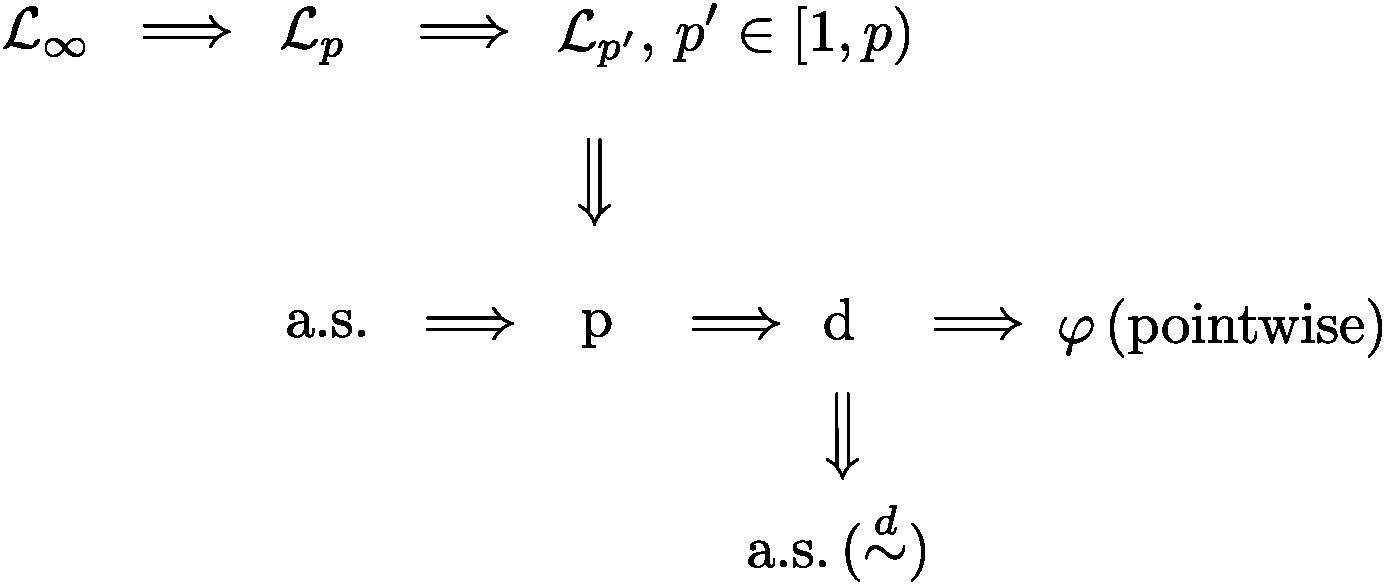
\includegraphics[width=0.6\linewidth]{figures/convergence_rv}
 \caption{Illustration of the relationships among different modes of convergence of random variables. 
         Convergence in $\mathcal{L}_\infty$ implies convergence in $\mathcal{L}^p$ for all $p\in[1,\infty)$
         which in turn implies convergence in $\mathcal{L}_{p'}$ for all $1\leq p' \leq p$ which implies 
         convergence in probability which implies convergence in distribution which implies 
         convergence of the characteristic functions (L\'evy's continuity theorem). 
         Convergence in distribution implies almost 
         convergence of a sequence of RVs $\{Y_k\}_k$ which have the same distribution as 
         $\{X_k\}_k$ ($Y_k \overset{d}{\sim} X_k$ and $Y \overset{d}{\sim} X$).
         }
\end{figure}


\subsection{Convergence in distribution}
\begin{enumerate}
\item (Convergence in distribution). The sequence of random variables $\{X_n\}_n$ with distributions 
      $\{\mu_n\}_n$ is said to converge in distribution of $X$ if $\{\mu_n\}_n$ converges weakly
      to $\mu$, the distribution of $X$.
      
\item (Slutsky's theorem). Let $X_k\to X$ in distribution and $Y_n\to c$ in probability, where $c$ is a constant.
      Then, 
      \begin{enumerate}[i.]
       \item $X_n + Y_n \to X + c$ in distribution
       \item $X_nY_n \to cX$ in distribution
       \item $X_n/Y_n \to X/c$ in distribution, provided that $c\neq 0$, $Y_n\neq 0$.
      \end{enumerate}
      
\item (Almost sure convergence). If $X_n\to X$ in distribution, we may find a probability space $\ofp$
      and random variables $Y$ and $(Y_n)_n$ so that $Y_n$ is equal in distribution to $X_n$,
      $Y$ is equal in distribution to $X$ and $Y_n\to Y$ almost surely.
      
\item (L{\'e}vy's continuity theorem)%
	  \footnote{Lecture notes 6.436J/15.085J by MIT, Available online at \url{https://goo.gl/7ZaHW9}.}. 
      Let $\{X_k\}_k$ be a sequence of random variables with characteristic functions $\varphi_k(t)$ and let $X$ be a random variable with characteristic function $\varphi(t)$. It $X_k$ converges to $X$ in distribution then $\varphi_k \to \varphi$ point-wise. Conversely, if $\varphi_k \to \varphi$ and $\varphi$ is continuous at $0$, then $\varphi$ is the characteristic function of a random variable $X$ and $X_k\to X$ in distribution.
      the 
\item (Scheff\'e's theorem for density functions).\footnote{S. Sagitov, ``Weak Convergence of Probability Measures,'' 2013, Available at: \url{https://goo.gl/m4Qi5i}}
Let $\prob_n$ and $\prob$ have densities $f_n$ and $f$
      with respect to a measure $\mu$. If $f_n \to f$ $\mu$-a.s., then $\prob_n \to \prob$ in the total 
      variation metric and, as a result,  $\prob_n \to \prob$ weakly.
      
\item (Continuous mapping theorem). For a (almost everywhere) continuous function $g$, if the sequence $\{X_k\}_k$ 
      converges in distribution to $X$, then $\{g(X_k)\}_k$ converges in distribution to 
      $g(X)$.
      
\item (Convergence in probability $\Rightarrow$ in distribution). If $\{X_k\}_k$ converges in probability,
      then it converges in distribution to the same limit.
      
\item (In distribution $\not\Rightarrow$ in probability). There are sequences which converge in distribution,
      but not in probability. For example: On the space $([0,1], \mathcal{B}_{[0,1]},\lambda)$, let $X_{2n}(\omega)=\omega$
      and $X_{2n-1}(\omega) = 1-\omega$. Then all $X_k$ have the same distribution, but the sequence does not 
      converge in probability. As a second example, the sequence $X_n=X$ where $X$ follows the Bernoulli distribution
      with parameter $\frac{1}{2}$, converges in distribution to $1-X$, but not in probability.
      
\item (Polya-Cantelli lemma)\footnote{Lecture notes of M. Banerjee, Available at: \url{http://dept.stat.lsa.umich.edu/~moulib/ch2.pdf}}. If $X_n\to X$ in distribution, $F_n$ are the distribution function of $X_n$ and 
      $X$ has the \textit{continuous} distribution function $F$, then $\|F_n - F\|_\infty \dfn \sup_{x}|F_n(x) - F(x)| \to 0$
      as $n\to\infty$.
      
\item (Delta method). Let \(X\) be a real-valued random variable and 
\(X_n\) be a sequence of real-valued random variables with 
\(
      n^c (X_n - \theta) \to X,
\)
in distribution for some $c>0$. 
Let $g:\Re\to\Re$ be function which is differentiable at $\theta$. Then,
\(
      n^c(g(X_n) - g(\theta)) \to g'(\theta)X.
\)\footnote{See the lecture notes at \url{http://personal.psu.edu/drh20/asymp/fall2006/lectures/}, Chap. 5.
 The proof makes use of Taylor's first-order expansion and Slutsky's theorem.}
\end{enumerate}



\subsection{Tail events and 0-1 Laws}
\begin{enumerate}

 \item (Simple 0-1 law). Let $\{E_n\}$ be a sequence of independent events. Then $\prob[\limsup_n E_n]\in \{0,1\}$.
 \item (Unions of $\sigma$-algebras). Let $\F_1$, $\F_2$ be two $\sigma$-algebras on a nonempty set $X$.
       The $\sigma$-algebra generated by the sets $E_1\cup E_2$ with $E_1\in\F_1$ and $E_2\in\F_2$ is 
       denoted by $\F_1 \vee \F_2$
 
 \item (Tail $\sigma$-algebra). Let $(\F_n)_{n}$ be a sequence of sub-$\sigma$-algebras of $\F$.
       The $\sigma$-algebra $T_n\dfn \bigvee_{m>n}\F_m$ encodes the information about the future 
       after $n$ and $T=\bigcap_n T_n$ is the \textit{tail $\sigma$-algebra} which encodes the 
       information of the end of time. 
       
 \item (Events in the tail $\sigma$-algebra). For a process $(E_n)_n$ be a sequence of events. 
       The associated tail $\sigma$-algebra $T$ is $\bigcap_n \sigma(\{E_k\}_{k\geq n})$.
       The event $\limsup_n E_n$ is in $T$.
 
 \item (Kolmogorov's zero-one law). Let $(\F_n)_n$ be a sequence of \textit{independent}
       $\sigma$-algebras on a nonempty set $X$ and let $T$ be the tail $\sigma$-algebra.
       We equip $(X,\F)$ with a probability measure $\prob$. For every $H\in T$,
       $\prob(H)\in\{0,1\}$.
 
 \item (Counterpart of the Borel-Cantelli lemma). 
 Let $\{E_n\}_{n\in\N}$ be a nested increasing sequence of events in $\ofp$, that is 
 $E_k\subseteq E_{k+1}$ and let $E_k^c$ denote the complement of $E_k$.
 Infinitely many $E_k$ occur with probability $1$ if and only if there is an increasing sequence 
 $t_k\in\N$ such that
 \[
  \sum_k \prob[A_{t_{k+1}}\mid A_{t_k}^c]  = \infty.
 \] 
 
 \item (L\'evy's zero-one law). Let $\Ff=\{\F_k\}_{k\in\N}$ be any filtration of $\F$ on $\ofp$ and
 $X\in\mathcal{L}_1\ofp$. Let $\F_\infty$ be the minimum $\sigma$-algebra generated by $\Ff$. Then
 \[
  \E[X\mid \F_k] \to \E[X\mid \F_\infty], 
 \]
 both in $\mathcal{L}_1\ofp$ and $\prob$-a.s.
\end{enumerate}



\subsection{Laws of large numbers and CLTs} 
\begin{enumerate}
  \item (Weak law of large numbers). Also known as Bernoulli's theorem. Let $\{X_k\}_k$ be
       a sequence of independent identically distributed random variables, each having a 
       finite mean $\E[X_k]=\mu$ and finite variance $\sigma^2$. Define 
       $\bar{X}_k=\nicefrac{1}{k}(X_1+\ldots+X_k)$. Then $\bar{X}_k\to \mu$ in probability.
   \item (Strong law of large numbers). Let $\{X_k\}_k$ and $\bar{X}_k$ be as above.
         Then $\bar{X}_k\to \mu$ almost surely.    
   \item (Uniform law of large numbers).  Let $f(x,\theta)$ be a function defined over
         $\theta\in\Theta$. For fixed $\theta$ and 
         a random process $\{X_k\}_k$ define $Z_k^\theta \dfn f(X_k, \theta)$. Let 
         $\{Z_k^\theta\}_k$ be a sequence of independent and identically distributed 
         random variables, such that the sample mean converges in probability to $\E[f(X, \theta)]$. 
         Suppose that (i) $\Theta$ is compact, (ii) $f$ is continuous 
         in $\theta$ for almost all $x$ and measurable with respect to $x$ for each $\theta$,
         (iii) there is a function $g$ such that $\E[g(X)]<\infty$ and $\|f(x,\theta)\| \leq g(x)$ 
         for all $\theta\in\Theta$. Then, $\E[f(X,\theta)]$ is continuous in $\theta$ and
         \[
          \sup_{\theta\in\Theta}\left\| 
	    \bar{Z}^\theta_k - \E[f(X,\theta)] 
          \right\|
          \overset{a.s.}{\longrightarrow} 0
         \]

   \item (Lindeberg-L{\'e}vy central limit theorem). Let $\{X_k\}_k$ be iid, finite mean and variance 
         and $\bar{X}_k$ as above. Then
         \[
          \frac{\bar{X}_k-\mu}{\sqrt{n}} \overset{d}{\longrightarrow} \mathcal{N}(0, \sigma^2),
         \]
         where \(\mathcal{N}(0, \sigma^2)\) is the normal distribution is zero mean and variance \(\sigma^2\)
         (See Section \ref{sec:normal_distribution}).

   \item (Lyapunov central limit theorem). Let $\{X_k\}_k$ be a sequence of independent random variables
         with $\E[X_k]=\mu_k$ and finite variance $\sigma_k^2$. Define $s_k^2 = \sum_{i=1}^{k}\sigma_i^2$.
         If for some $\delta>0$, the following condition holds (Lyapunov's condition)%
         \footnote{In practice it is usually easiest to check Lyapunov's condition for $\delta=1$. 
                   If a sequence of random variables satisfies Lyapunov's condition, then it also 
                   satisfies Lindeberg's condition. The converse implication, however, does not hold.}:
         \[
          \lim_{k\to\infty} \frac{1}{s_k^{2+\delta}}\sum_{i=1}^{k}\E\left[ 
          |X_i - \mu_i|^{2+\delta}
          \right]=0,
         \]
	 then,
	 \[
	  \frac{1}{s_k}\sum_{i=1}^{k}(X_i - \mu_i) \overset{d}{\longrightarrow} \mathcal{N}(0, 1).
	 \]

 \item (Law od iterated logarithm). Let \((X_k)_{t\in\N}\) be independent identically 
       distributed random variables and let \(S_k{}\dfn{} X_1 + \ldots + X_k\). Then,
       \[
        \limsup_{k}\frac{S_k}{\sqrt{2k\ln \ln k}} = 1,
       \]
       and convergence is in the almost sure sense.

 \item (Delta method). Let \((X_n)_n\) be a sequence of random variables satisfying
 \[
  \sqrt{n}(X_n - \theta) \overset{d}{\to} \mathcal{N}(0,\sigma^2).
 \]
 Let \(g:\Re\to\Re\) be a function which is differentiable at \(\theta\) and \(g'(\theta)\neq 0\).
 Then,
 \[
  \sqrt{n} (g(X_n) - g(\theta)) \overset{d}{\to} \mathcal{N}(0, \sigma^2[g'(\theta)]^2)
 \]

 

\end{enumerate}



\section{Standard Distributions}
\subsection{Uniform distribution}
\begin{enumerate}
 \item (Definition). A random variable \(X:\Omega\to[a,b]\), \(a<b\), is said to follow the 
       uniform distribution, denoted as \(X\sim U(a,b)\), if its cumulative distribution 
       function is
       \[
        F_X(x) = \prob[X \leq x] = \begin{cases}
                                    0,&\text{ for } x<a\\
                                    \nicefrac{x-a}{b-a},&\text{ for } a \leq x < b\\
                                    1,&\text{ for } x\geq b\\
                                   \end{cases}
       \]
       The probability density function of \(X\) is
       \[
        f_X(x) = \begin{cases}
                  \nicefrac{1}{b-a},&\text{ for } x\in [a,b]\\
                  0,&\text{ otherwise}
                 \end{cases}
       \]
       The distribution \(U(0,1)\) is called the \textit{standard uniform distribution}.
 \item (Characteristics). For \(X\sim U(a,b)\), the expectation of \(X\) is \(\E[X] = \frac{a+b}{2}\), 
       and its variance is \(\mathrm{Var}[X] = \nicefrac{1}{12}(b-a)^2\).
 \item (Probability integral transform). Let \(X\) be a real-valued random variable which has 
       a continuous distribution with cumulative distribution function \(F_X\). Then, the random 
       variable \(Y = F_X(X)\), that is, \(Y(\omega) = F_X(X(\omega))\) follows the standard 
       uniform distribution.
 \item (Inverse probability integral transform). Let \(Y\sim U(0,1)\) and let \(X\) be a 
       random variable with cumulative distribution function \(F_X\). Then \(F_X^{-1}(Y)\) 
       has the same distribution as \(X\).
\end{enumerate}


\subsection{Normal distribution}\label{sec:normal_distribution}
\begin{enumerate}
 \item (Definition: univariate case). For a real-valued random variable \(X\), the PDF \(f_X\) of the normal 
       distribution on \(\Re\) with parameters \(\mu\) and \(\sigma\) is given by
 \[
  f_X(x) = \frac{1}{\sqrt{2\pi \sigma^2}}\exp\left(-\frac{(x-\mu)^2}{2\sigma^2}\right),
 \]
 and cumulative distribution function 
 \[
  F_X(x) = \frac{1}{2}\left( 1 + \operatorname{erf}\left(\frac{x-\mu}{\sqrt{2} \sigma}\right) \right).
 \]
 We write \(X\sim \mathcal{N}(\mu, \sigma)\) to denote that \(X\) follows the normal distribution 
 with parameters \(\mu\) and \(\sigma\).

 \item (Characteristics). The mean, median and mode of \(\mathcal{N}(\mu, \sigma)\) are equal to \(\mu\).
       Its variance is \(\sigma^2\) and its MGF is \(M_X(z) = \exp(\mu z + \sigma^2 z^2/2)\)

 \item (Sum and scalar product of normals). Let \(X\sim\mathcal{N}(\mu_X, \sigma_X^2)\) and 
       \(Y\sim\mathcal{N}(\mu_Y, \sigma_Y^2\) be two independent random variables. 
       Then \(X+Y\sim\mathcal{N}(\mu_X+\mu_Y, \sigma_X^2 + \sigma_Y^2)\).
       If \(X\) and \(Y\) are jointly normally distributed random variables, then 
       \(X+Y\) is normally distributed and \(E[X+Y] = \mu_X + \mu_Y\) and 
       \(\sigma_{X+Y} = \sqrt{\sigma_X^2 + \sigma_Y^2 + 2\rho\sigma_X\sigma_Y}\), where 
       \(\rho\) is the correlation between \(X\) and \(Y\).
       For any \(\alpha\in\Re\), \(\alpha X\sim \mathcal{N}(\alpha\mu_X, \alpha^2\sigma_X^2)\).
       
 \item (Multivariate normal distribution). The multivariate variant of the normal distribution,
       denoted by $\mathcal{N}(\mu, \Sigma)$ with $\mu\in\Re^n$ and $\Sigma\in\Re^{n\times n}$,
       symmetric positive semi-definite, is supported on $\mu + \operatorname{im}(\Sigma)$
       and PDF 
       \[
        p_X(x) = |2\pi \Sigma|^{-\nicefrac{1}{2}}\exp\left(-\tfrac{1}{2}(x-\mu)^{\top}\Sigma(x-\mu)\right).
       \]

 
 \item (Linear transformation). Let $X\sim \mathcal{N}(\mu,\Sigma)$, $\mu\in\Re^n$, $\Sigma\in\Re^{n\times n}$ 
       and $Y=AX+b$ for constant $A$ and $b$. Then $Y\sim \mathcal{N}(A\mu+b, A\Sigma A')$.
 \item (Conditioning). Let $X_1$, $X_2$ be two random variables with values in $\Re^{n_1}$ and $\Re^{n_2}$
       respectively. Suppose that
\begin{equation*}
        \begin{bmatrix}
         X_1\\X_2
        \end{bmatrix}
{}\sim{}
	\mathcal{N}\left(
	\begin{bmatrix}
         \mu_1\\\mu_2
        \end{bmatrix},
        \begin{bmatrix}
         \Sigma_{11} & \Sigma_{12}\\
         \Sigma_{21} & \Sigma_{22}
        \end{bmatrix}
        \right).
\end{equation*}
Then, \(\E[X_1\mid X_2=x_2] \sim \mathcal{N}(\mu(x_2), \Sigma)\) with 
\begin{align*}
	\mu(x_2) 
{}={}& 
	\mu_1 
{}+{}
	\Sigma_{12}\Sigma_{22}^{-1}(x_2{}-{}\mu_2),
\\
	\Sigma 
{}={}&
	\Sigma_{11}
{}-{}
	\Sigma_{12}\Sigma_{22}^{-1}\Sigma_{21}.
\end{align*}
\end{enumerate}


\subsection{Binomial distribution}\label{sec:binomial_distribution}
\begin{enumerate}
 \item (Definition). For \(n\in\N\) and \(p\in[0,1]\), we say that a random variable 
       \(X:\Omega\to\{0,\ldots, n\}\) follows the Binomial distribution, we denote 
       \(X \sim B(n,p)\), if its probability mass function is
       \[
        \prob[X = k] = {n \choose k} p^k (1-p)^{n-k},
       \]
       where \({n \choose k} = \frac{n!}{k!(n-k)!}\)
 \item (Characteristics). If \(X \sim B(n,p)\), then \(\E[X]=np\), the median of \(X\) 
       is either \(\lfloor np \rfloor\) or \(\lceil np \rceil\), its variance is 
       \(\mathrm{Var}[X] = np(1-p)\) and moment generating function (MGF) of \(X\) is 
       \(M_X(z) = (1-p+pe^z)^n\). The cumulative probability function of \(X\) is given 
       in terms of the regularized incomplete beta function
       \[
        \prob[X \leq x] = I_{1-p}(n-k, k+1)
       \]
 \item (Sum of independent Binomials). Let \(X\sim B(n,p)\) and \(Y\sim B(m,p)\) be 
       independent random variables. Then, \(X+Y\) follows the Binomial distribution
       \(B(n+m, p)\).
       
 \item (Binomial sum variance inequality). Let \(X\sim B(n,p)\) and \(Y\sim B(n',p')\) 
       be two random variables, not necessarily independent. Let \(S=X+Y\). Then,
       \[
        \mathrm{Var}[S] \leq \E[S]\frac{1-\E[S]}{n+n'}.
       \]
       
 \item (De Moivre-Laplace theorem). For large \(n\) and \(k\) in the neighbourhood of \(np\),
       it is 
       \[
        {n \choose k} p^k (1-p)^{n-k} \approxeq \frac{1}{\sqrt{2\pi n p (1-p)}}e^{-\frac{(k-np)^2}{2np(1-p)}}.
       \]
       As an example, consider the experiment of tossing \(n\) coins a large number of times 
       and observing the number of heads each time. Then, as \(n\) grows large, the shape of 
       the distribution of the number of heads approaches that of the normal distribution.
\end{enumerate}


\subsection{Poisson distribution}
\begin{enumerate}
 \item (Definition). We say that a random variable \(X:\Omega\to\N\) follows the Poisson distribution
       with parameter \(\lambda\) if its probability mass function is
       \[
        \prob[X = k] = \frac{\lambda^k e^{-\lambda}}{k!}
       \]
       We denote \(X\sim\mathrm{Poisson}(\lambda)\).
 \item (Characteristics). If \(X\sim\mathrm{Poisson}(\lambda)\), then \(\E[X]=\lambda\), 
       \(\mathrm{Var}[X]=\lambda\) and the moment generating function (MGF) of \(X\) is 
        \(M_X(z) = \exp(\lambda (e^z - 1))\). The median of \(X\) is in the interval 
        \([\lambda - \ln 2, \lambda + \nicefrac{1}{3}\).
        
 \item (Sum of independent Poissons). Let \(X_i\), \(i\in\N_{[1,N]}\), be independent random 
       variables with \(X_i\sim\mathrm{Poisson}(\lambda_i)\). Define the random variable 
       \(S = X_1 + \ldots + X_N\) and \(\lambda = \lambda_1 + \ldots + \lambda_N\), then
       \(S \sim \mathrm{Poisson}(\lambda)\).
       
 \item (Raikov's theorem). If the sum of two independent nonnegative random variables, 
       \(X\) and \(Y\), follows the Poisson distribution, then both \(X\) and \(Y\)
       follow the Poisson distribution.
       
 \item (Law of rare events/Poisson limit theorem). Let \((p_n)_{n\in\N}\) be a sequence of 
       numbers in \([0,1]\) such that \(np_n\) converges to a limit \(\lambda\). Then
       \[
        \lim_{n\to\infty}\smashunderbracket{{n \choose k} p_n^k (1-p_n)^{n-k}}{\text{Binomial PMF}} 
        =
        \smashunderbracket{e^{-\lambda}\frac{\lambda^k}{k!}}{\text{Poisson PMF}}.
       \]
 \item (Large \(\lambda\)). For large values of \(\lambda\), e.g., \(\lambda>10^3\), the 
       normal distribution \(\mathcal{N}(\lambda, \lambda)\), is considered 
       a good approximation to \(\mathrm{Poisson}(\lambda)\).

\end{enumerate}

\chapter{Multivariate distributions}
\section{Multivariate random variables}
\begin{enumerate}
 \item (Multivariate CDF). The cdf of a random variable \(X:\ofp\to\Re^d\) is the function 
       \begin{align*}
        F_X(x_1, \ldots, x_d) =& \prob[X_1\leq x_1, \ldots, X_d \leq x_d]
        \\
        =& \prob\left[\bigcap_{i=1,\ldots, d} \{X_i \leq x_i\}\right]
       \end{align*}
 \item (Multivariate CDF properties). The cdf \(F_X\) of a random variable \(X:\ofp\to\Re^d\)  
       has the following properties
       \begin{enumerate}[i.]
        \item It is monotonically decreasing with respect to each variable
        \item It is right-continuous with respect to each variable
        \item \(0 \leq F_X(x_1, \ldots, x_d)\leq 1\) for all \(x_1,\ldots, x_d\in\Re\)
        \item \(\lim_{x_1,\ldots, x_d\to\infty} F_X(x_1, \ldots, x_d) = 1\)
        \item \(\lim_{x_i\to-\infty} F_X(x_1, \ldots, x_d) = 0\) for all \(i\in\N_{[1,d]}\)
       \end{enumerate}
 \item (Expectation and variance). The expectation of a random variable \(X:\ofp\to\Re^d\), 
       \(X = (X_1, X_2,\ldots, X_d)\) is defined as 
       \[
        \E[X] = (\E[X_1], \E[X_2], \ldots, \E[X_d])
       \]
       And the \textit{variance-covariance matrix} of \(X\) is 
       \[
        \mathrm{V}(X) = \E[(X-\E[X])(X-\E[X])^{\top}],
       \]
       which is the multivariate counterpart of variance.


\end{enumerate}

\section{Copulas}
\subsection{Sklar's theorem}
\begin{enumerate}
 \item (Definition). Let \(X\) be an \(d\)-dimensional random variable, with 
       \(X(\omega) = (X_1(\omega), X_2(\omega), \ldots, X_d(\omega)\) with continuous marginal CDFs
       \(F_{X_i}(x) = \prob[X_i \leq x]\). By the probability integral transform, the random variable 
       \(U=(U_1,\ldots, U_d)\) defined as 
       \[
        U_i = F_{X_i}(X_i), 
       \]
       for \(i=1,\ldots, d\), has uniformly distributed marginals, that is, 
       \(U_i \sim U(0,1)\). The \textit{copula} of \(X\) is the joint cumulative distribution 
       function of \(U\), that is 
       \begin{align*}
        C(u_1, \ldots, u_d) 
	  =& \prob[U_1 \leq u_1, \ldots, U_d \leq u_d]
	  \\
	  =& \prob[X_1 \leq F_{X_1}^{-1}(u_1), \ldots, X_d \leq F_{X_d}^{-1}(u_d)].
       \end{align*}
       A \(d\)-dimensional copula is a function \(C:[0,1]^d\to[0,1]\)
       which is a joint cumulative distribution function of a \(d\)-dimensional random variable 
       on the \([0,1]^d\) with uniform marginals.
 \item (Sklar's theorem). Every multivariate CDF, \(H(x_1, \ldots, x_d) = \prob[X_1\leq x_1, \ldots, X_d \leq x_d]\),
       can be expressed in terms of its marginals, \(F_{X_i}(x) = \prob[X_i \leq x]\), and a copula \(C:[0,1]^d\to[0,1]\), 
       that is 
       \[
        H(x_1, \ldots, x_d) = C(F_{X_1}(x_1), \ldots, F_{X_d}(x_d)).
       \]
       If the multivariate distribution has a PDF \(h\), then there is a function \(c\)
       called the density copula and 
       \[
        h(x_1,\ldots, x_d) = c(F_{X_1}(x_1), \ldots, F_{X_d}(x_d)) f_1(x_1)\cdot \ldots \cdot f_d(x_d).
       \]
       Conversely, given a copula \(C:[0,1]^d\to[0,1]\) and marginal distributions 
       \(F_{X_i}\), there is a \(d\)-dimensional CDF as described above.
 \item (Characterization). A function \(C: [0,1]^d\to[0,1]\) is a copula if and 
       only if it satisfies the following properties
       \begin{enumerate}[i.]
        \item For every \(j\in\N_{[1,d]}\), \(C(1,\ldots, 1, t, 1, \ldots, 1) = t\)
        \item \(C\) is isotonic (order preserving), that is, \(C(u) \leq C(u')\) whenever
        \(u \leq u'\) in the sense \(u_i \leq u'_i\) for all \(i\in\N_{[0,d]}\)
        \item \(C\) is \(d\)-nondecreasing, that is, for every hyperrectange \(B\), 
        the \(\d C\)-volume \(B\) is nonnegative, that is
        \[
         \int_{B}\d C \geq 0,
        \]
        where \(\d C\) is treated as a measure.
       \end{enumerate}
       
 \item (Characterization of two-dimensional copulas). A two-dimensional copula 
       \(C: [0,1]^2 \to [0,1]\) satisfies the following properties
       \begin{enumerate}[i]
        \item for every \(u\in[0,1]\), \(C(u,0) = C(0,u) = 0\)
        \item for every \(u\in[0,1]\), \(C(u, 1) = C(1, u) = u\)
        \item for all \(u,u',v,v' \in [0,1]\) with \(u\leq u'\) and \(v\leq v'\)
        \[
         C(u', v')  - C(u', v) - C(u,v') + C(u,v) \geq 0
        \]
       \end{enumerate}
 
 \item (Properties of copulas). A copula \(C:[0,1]^d\to[0,1]\) possesses the following 
       properties
       \begin{enumerate}[i.]
        \item \(C(u_1, \ldots, u_d)=0\) if there is an \(i_0\in\N_{[1,d]}\) so that \(u_{i_0}=0\)
        \item \(C\) is nonexpansive in the following sense
        \[
         |C(u) - C(v)| \leq \sum_{i=1}^{d}|u_i - v_i|
        \]

       \end{enumerate}


 \item (Fr{\'e}chet-Hoeffding copula bounds). For any copula \(C:[0,1]^d\to[0,1]\), 
       \[
        W(u_1,\ldots, u_d) \leq C(u_1,\ldots, u_d) \leq M(u_1,\ldots, u_d),
       \]
       where 
       \[
        W(u_1,\ldots, u_d) \dfn \max\{0, 1-d+\textstyle\sum_{i=1}^{d}u_i\},
       \]
       and
       \[
        M(u_1,\ldots, u_d) = \min\{u_1,\ldots, u_d\}.
       \]
       The upper bound is sharp, \(M\) is always a copula and equality is attained
       for comonotone random variables. 
\end{enumerate}

\subsection{Examples of copulas}


\chapter{Stochastic Processes}\label{sec:stoch-proc}
\section{General}\label{sec:stoch-proc-general}
\begin{enumerate}
 \item (Stochastic process). Let $\T \subseteq \barre$ (e.g., $T=\N$ or $T=\barre$). A random process is 
       a sequence/net $(X_n)_{n\in \T}$ of (real-valued) random variables on a probability space $\ofp$.

 \item (Version). Let \(T=[0,\infty)\) be a time index set and \((X_t)_t\), \((Y_t)_t\) be two stochastic processes 
                  on \(\ofp\). We say that  \((X_t)_t\) is a version of \((Y_t)_t\)  if 
                  \[
                   X_t = Y_t, \prob{\text{-a.s. for all }} t\in T,
                  \]
                  that is, \(\prob[\{\omega \mid X_t(\omega) = Y_t(\omega)\}] = 1\) for all \(t\in T\).

                  
 \item (Centered). Let \((X_t)_t\) be a real-valued stochastic process with \(t\in[a,b]\).
       We say that \((X_t)_t\) is centered if \(\E[X_t]=0\) for all \(t\in[a,b]\).
       
 \item (Mean-square continuous). Let \((X_t)_t\) be a real-valued stochastic process with \(t\in[a,b]\).
       We say that \((X_t)_t\) is mean-square continuous if 
       \[
        \lim_{\epsilon \to 0}\E[(X_{t+\epsilon}-X_t)^2]=0,
       \]
       for all \(t\in[a,b]\).

 \item (Auto-correlation function). Let \((X_t)_{t\in T}\) be a stochastic process. Define 
       the function \(R_X:T\times T\to \Re\) as 
       \[
        R_X(s,t) = \E[X_s X_t].
       \]
       This function is called the auto-correlation function of \((X_t)_t\).
       
 \item (Mean-square continuity criterion). A stochastic process \((X_t)_{t\in[a,b]}\) is
       mean-square continuous if and only if its auto-correlation function, \(R_X\), is 
       continuous on \([a,b]\times [a,b]\).
       
 \item (Filtrations). A filtration is an increasing sequence of sub-$\sigma$-algebras of $\F$. The space 
       $(\Omega, \F, (\F_t)_{t\in \T}, \prob)$ is called a filtered probability space. The filtration 
       $\F_t = \sigma(\{X_s; s\in \T, s\leq t\})$ is called the filtration \textit{generated by $(X_n)_{n\in \T}$}.
       We say that $(X_n)_n$ is adapted to a filtration $(\F_n)_n$ if for all $n\in \T$, $X_n$ is $\F_n$-measurable.
       
 \item (Stopping times). Let $(\F_n)_n$ be a filtration on $\ofp$ and define $\overline{\T} \dfn \T \cup \{+\infty\}$.
       A random variable $T: \Omega \to \overline{\T}$ is called a stopping time if
       \[
        \{\omega {}\mid{} T(\omega) \leq t\} \in \F_t,
       \]
      for all $t\in \T$. This is equivalent to requiring that the process $Z_t = 1_{T \leq t}$ is adapted to $(\F_t)_{t\in \T}$.
      
 \item (A useful property). For any stochastic process $(X_n)_{n\in\N}$, we have
 \[
  \prob\left(\max_{i\leq k}|X_i|>\epsilon\right) = \prob\left(\sum_{i=0}^{k}X_i^2 \cdot  1_{\{|X_i|>\epsilon\}}>\epsilon^2\right).
 \]
 \item \label{it:kolmogorov-cont-theorem} 
       (Kolmogorov's continuity theorem). Let \((X_t)_t\) be an \(\Re^{n}\)-valued stochastic process on \(\ofp\).
       Suppose that \((X_t)_t\) is such that for all \(t>0\) there 
       are positive constants \(\alpha, \beta, L\) such that 
       \[
        \E[\|X_{\tau} - X_{\tau'}\|^\alpha] \leq L |\tau' - \tau|^{1+\beta},
       \]
       for \(\tau \geq 0\) and \(\tau' \leq t\). Then, there is a continuous version of \(X\).
\end{enumerate}


\section{Random walk}
\begin{figure}
 \centering
 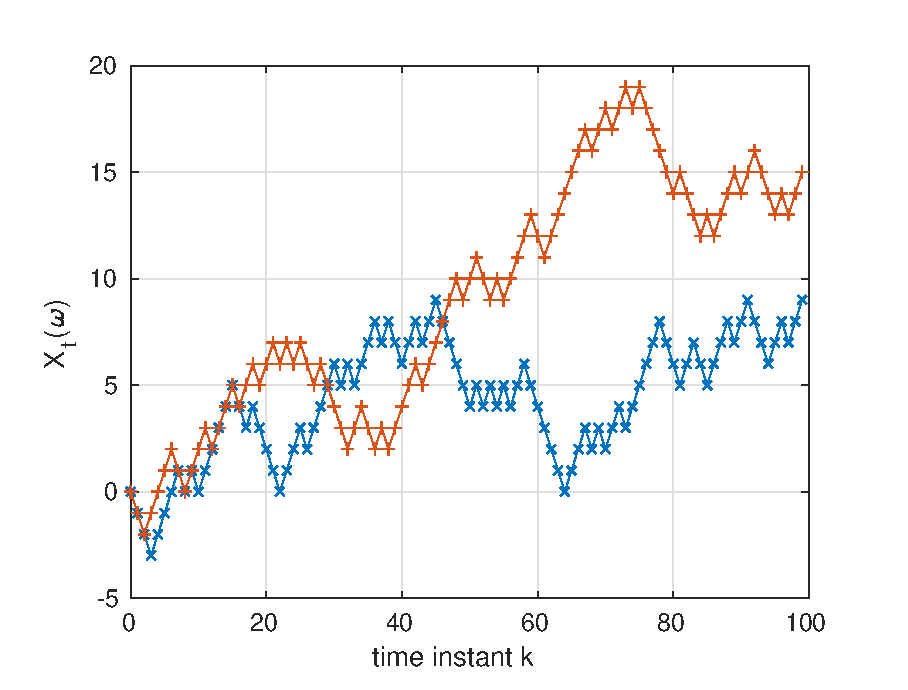
\includegraphics[width=0.55\textwidth]{figures/randomWalk}
 \caption{Random walk: two different paths, \((X_t(\omega_1))_t\) and \((X_t(\omega_2))_t\).}
 \label{fig:random_walk}
\end{figure}
\begin{enumerate}
 \item (One-dimensional random walk). Take a sequence of independent random variables \((Z_{t})_{t\in\N}\) that take 
       values in \(\{-1, 1\}\), each with probability \(0.5\). Define a random process 
       \((X_t)_{t\in \N}\) with \(X_0=0\) and \(X_t = \sum_{i=1}^{t}Z_i\). The process \((X_t)_{t\in \N}\) is called
       a (one-dimensional) (simple) random walk on \(\mathbb{Z}\). A random walk is shown in Figure~\ref{fig:random_walk}.              
       
       More generally, a random walk can be such that \(p\dfn\prob[Z_{t+1} - Z_{t} = 1] \neq \prob[Z_{t+1} - Z_{t} = -1]\).
       
 \item (Characteristics). The expectation of random walk \((X_t)_{t\in\N}\) with \(p=\nicefrac{1}{2}\) 
       is \(\E[X_t]=0\) and its variance is \(\E[X_t^2] = t\). Additionally,
       \[
        \lim_{t}\frac{\E[X_t]}{\sqrt{t}} = \sqrt{\frac{2}{\pi}}.
       \]
 \item (Distribution of \(X_t\)). Let \((X_t)_t\) be a one-dimensional random walk with 
       \(p\dfn \prob[X_{t+1} - X_{t} = 1]\) and define \(q \dfn 1-p\). 
       For \(t\in\N\), \(t\geq 1\), random variables \(X_t\) take values on 
       \(\mathcal{X}_t \dfn \{-t, -t+2, \ldots, t-2, t\}\) and their distribution is given by
       \[
        \prob[X_t = m] = {t \choose \tfrac{1}{2}(t+m)} p^{\tfrac{1}{2}(t+m)} q^{\tfrac{1}{2}(t-m)},
       \]
       for all \(m \in \mathcal{X}_t\)
       This is the Binomial distribution on \(\mathcal{X}_t\) with parameter \(p\) 
       (See definition in Section \ref{sec:binomial_distribution}).
 \item (Maximum of random walk). Let \(X_t\) be a simple symmetric random walk (with \(p=0.5\)
       and define \(M_t = \max_{t'\leq t}X_{t'}\). Then, \(M_0=0\), the support of \(M_t\) is 
       \(\{0,1,\ldots, t\}\) and 
       \[
        \prob[M_t = m] = \prob[X_t = m] + \prob[X_t = m+1] = {t \choose {\lfloor \tfrac{t+m+1}{2}\rfloor} }2^{-t}
       \]

 \item (Gaussian random walk). Take a sequence of independent random variables \(Z_{t}\) with \(Z_t\sim\mathcal{N}(\mu, \sigma^2)\).
       The random process \((X_t)_t\) with \(X_0=0\) and \(X_t = Z_1+\ldots+Z_t\) is called Gaussian random walk.
       It is \(X_t\sim \mathcal{N}(t\mu, t\sigma^2)\).
\end{enumerate}

\section{Martingales}
\begin{enumerate}
 \item (Martingale). A random process $(X_n)_n$ is called a \textit{martingale} if 
		     $\E[|X_n|]<\infty$ and $\E[X_{n+1}{}\mid{}X_1,\ldots, X_n]=X_{n}$.
 \item (Martingale examples). The following are common examples of martingales:
  \begin{enumerate}
   \item Let $(X_n)_n$ be a sequence of iid random variables with mean $\E[X_n]=\mu$. Then
         $Y_n = \sum_{i=1}^{n}(X_i-\mu)$ is a martingale.
   \item Let $(X_n)_n$ be a sequence of iid random variables with mean $\E[X_n]=1$ and finite
         variance. Define a sequence of random variables with \(Y_0=0\) and 
         \(Y_n = X_0 X_1 \cdot \ldots \cdot X_n\). Then, by the Cauchy-Swartz inequality,
         \(Y_n\) is a martingale.
   \item If $(X_n)_n$ is a sequence of iid random variables with mean $1$, then 
         $Y_n = \prod_{i=1}^{n}X_i$ is a martingale.
   \item If $(X_n)_n$ is a sequence of random variables with finite expectation and 
         $\E[X_n{}\mid{}X_1,\ldots,X_{n-1}]=0$, then $Y_n=\sum_{i=0}^{n}X_i$ is a 
         martingale.
   \item (The classical martingale). The fortune of a gambler is a martingale in a fair game.
  \end{enumerate}
 \item (Sub- and super-martingales). A random process $(X_n)_n$ is called a \textit{super-martingale} if 
		     $\E[|X_n|]<\infty$ and $\E[X_{n+1}{}\mid{}X_1,\ldots, X_n]\leq X_{n}$. Likewise, it 
		     is a \textit{sub-martingale} if $\E[|X_n|]<\infty$ and $\E[X_{n+1}{}\mid{}X_1,\ldots, X_n]\geq X_{n}$.
 \item (Stopping time). Let $\{Z_k\}_k$ be a random process and $T$ a stopping time. 
       Define $X_k(\omega) = Z_{k\wedge T(\omega)}$, that is
       \[
        X_k(\omega) = \begin{cases}
                       Z_k(\omega),&\text{if }k \leq T(\omega)\\
                       Z_{T(\omega)}(\omega),&\text{otherwise}
                      \end{cases}
       \]
       If $Z$ is a (sub-) martingale, then $X$ is a (sub-) martingale too.
 \item (Doob's optimal stopping theorem). Let \((X_n)_n\) be a super-martingale and \(T\) be a stopping 
       time. Then \(X_T\) is integrable and \(\E[X_T] \leq \E[X_0]\) in each of the following cases
	  \begin{enumerate}[i.]
	   \item \(T\) is bounded 
	   \item \(X\) is bounded and \(T\) is almost surely finite
	   \item \(E[T]<\infty\) and \((X_n)_n\) has (surely) bounded differences, i.e., there is an \(M>0\) such that
	    \[
	     |X_n(\omega) - X_{n-1}(\omega)| \leq M, 
	    \]
	   for all \(n\in\N\) and \(\omega\in\Omega\)
	   \item \(X_n\geq 0\) for all \(n\) and \(T\) is almost surely finite
	  \end{enumerate}

 \item (Martingale stopping).
 \item (Almost sure martingale convergence). Let $(X_n)_n$ be a martingale which is uniformly 
       bounded in $\mathcal{L}_1$, i.e., $\sup_n \E[|X_n|] < \infty$. Then, there is a $X\in\mathcal{L}_1(\mathcal{F}_\infty)$,
       so that $X_n\to X$ a.s., where $\mathcal{F}_\infty = \sigma(\mathcal{F}_n, n\geq 0)$.
 \item (Kolmogorov's sub-martingale inequality). Let $\{X_k\}_k$ be a nonnegative sub-martingale.
       Then, for $n\in\N_{>0}$ and $\alpha>0$,
       \[
        \prob\left[ \max_{k=1,\ldots, n}X_k \geq \alpha\right] \leq \frac{\E[X_n]}{\alpha}.
       \]
       \begin{enumerate}[i.]
        \item (Corollary 1). Let $\{X_k\}_k$ be a nonnegative martingale. 
              Then $\prob[\sup_{k\geq 1}X_k \leq \alpha]\leq\E[X_1]/\alpha$ for $\alpha>0$.
        \item (Corollary 2). Let $\{X_k\}_k$ be a martingale with $\E[X_k^2]< \infty$ for all $k\in\N_{>0}$. 
               Then, $\prob[\max_{k=1,\ldots, n}|X_k|\geq \alpha]\leq \E[X_n^2]/\alpha$ for all $n\in \N_{\geq 2}$
               and $\alpha>0$.
        \item (Corollary 3). Let $\{X_k\}_k$ be a nonnegative super-martingale. Then, for $n\in\N_{>0}$
              and $\alpha>0$, $\prob[\cup_{k\geq n}\{Z_k\geq \alpha\}]\leq\E[Z_n]/\alpha$.
       \end{enumerate}


 \item (Azuma-Hoeffding inequality for martingales with bounded differences). Let $(X_i)_i$
       be a martingale or a  super-martingale and $|X_k-X_{k-1}|<c_{k}$ almost surely. Then for all $N\in\N$
       and $t\in\Re$,
       \[
        \prob[X_N-X_0\geq t] \leq \exp \left(-\frac{t^2}{2\sum_{i=1}^{N}c_i^2}\right)
       \]
       If $(X_i)_i$ is a sub-martingale, 
       \[
        \prob[X_N-X_0\leq -t] \leq \exp \left(-\frac{t^2}{2\sum_{i=1}^{N}c_i^2}\right)
       \]

\end{enumerate}


\section{Brownian motion and Wiener processes}
\begin{enumerate}
 \item (Definition). A stochastic process \((X_t)_{t\in \Re_+}\) on \((\Re, \mathcal{B}(\Re))\) is 
 called Brownian motion if it is continuous and has stationary independent increments. A process 
 \((W_t)_{t\in\Re_+}\) is called a Wiener process if it is a Brownian motion with 
 \begin{enumerate}[i.]
  \item \(W_0 = 0\)
  \item \(\E[W_t] = 0\)
  \item \(\E[W_t^2] = t\) for all \(t\in\Re_+\)
 \end{enumerate}
  \item (Definition according to \O{}ksendal). Following Kolmogorov's extension theorem,
        for given time instants \(t_1, \ldots, t_k\) in a time set \(T\) (typically \(T=[0, \infty)\)),
        define the following proability measure on \(\Re^{nk}\)
        \[
         \nu_{t_1,\ldots, t_k}(F_1\times \cdots \times F_k)
         =
         \int_{F_1\times\cdots\times F_k}\hspace{-1.6em} p(t_1, x, x_1) p(t_2-t_1, x_2, x_1) \cdots p(t_k - t_{k-1}, x_{k-1}, x_{k})
         \d x_1 \d x_2 \cdots \d x_k,
        \]
	where \(p\) is the function
	\[
	 p(t, x, y) {}={} (2\pi t)^{-n/2}\exp\left(-\tfrac{\|x-y\|^2}{2t}\right).
	\]
	Let \(\ofp\) be the associated probability space from Kolmogorov's extension theorem 
	and let \((B_t)_t\) be an \(\Re^{n}\)-valued stochastic process with 
	\[
	 \prob[B_{t_1} \in F_1, \ldots, B_{t_k} \in F_k] = \nu_{t_1,\ldots, t_k}(F_1\times \cdots \times F_k).
	\]
	Such a process is a (version of) Brownian motion starting at \(x\).
 \item (Expectation and covariance). Let \((B_t)_{t\in T}\) be a Brownian motion starting at \(x\).
        Then \(\E[B_t] = x\) for all \(t\in T\). Let \(t_1, \ldots, t_k\) be time instants and 
        \(Z = (B_{t_1}, B_{t_2}, \ldots, B_{t_k})\) be an \(\Re^{nk}\)-valued random variable.
        Then,
        \[
        \operatorname{cov}[Z] = \begin{bmatrix}
                                 t_1 I_n & t_1 I_n & \cdots & t_1 I_n 
                                 \\
                                 t_1 I_n & t_2 I_n & \cdots & t_2 I_n
                                 \\
                                 \vdots & \vdots & \ddots & \vdots
                                 \\
                                 t_1 I_n & t_2 I_n & \cdots & t_k I_n 
                                \end{bmatrix}
        \]
	Observe that, as a result, we have
	\[
	 \E[(B_t - x)(B_s - x)] = n \min(s,t).
	\]
 \item (Existence of continuous version). The Brownian motion satisfies Kolmogorov's continuity theorem 
       (see item \ref{it:kolmogorov-cont-theorem} in Section \ref{sec:stoch-proc-general}) with \(\alpha = 4\), 
       \(\beta = 1\) and \(L = n(n+2)\). In particular, 
       \(
	      \E[\|X_{\tau} - X_{\tau'}\|^4] 
	{}={} 
	      n(n+2) |\tau' - \tau|^2.
	\)
 \item (Zero crossing). The Brownian motion crosses the time axis infinitely often in every time interval
       \((0, t)\) for \(t>0\).
       
 \item (Distribution of maximum). Let \(X_t\) be a Brownian motion and \(M_t = \max_{s \leq t} X_s\).
       Then, for all \(t>0\) and \(a>0\),
       \[
        \prob[M_t \geq a] = 2\prob[X_t \geq a] = 2(1-\Phi(a/\sqrt{t})).
       \]

 \item (Nowhere differentiable). For every \(\omega\in\Omega\), \(t\mapsto X_t(\omega)\) is 
        nowhere differentiable.
 \item (Orthogonal transformation). Let \(B_t\) be an \(n\)-dimensional Brownian motion starting at \(0\) and 
       \(U\) be an orthogonal matrix, \(UU^{\top} = I\). Them,
       \(\tilde{B}_t = UB_t\) is a Brownian motion.
 \item (Brownian scaling).   Let \(B_t\) be an \(n\)-dimensional Brownian motion and \(c>0\).
       Then, \(\hat{B}_t = \nicefrac{1}{c}B_{c^2 t}\) is a Brownian motion.       
 \item (Time inversion). Let \(B_t\) be an \(n\)-dimensional Brownian motion starting at \(0\) and 
       \((\breve{B}_t)_t\) is a process with \(\breve{B}_0 = 0\) and \(\breve{B}_t = t B_{1/t}\).
       Then \(\breve{B}\) is a Brownian motion.
\end{enumerate}



\section{Markov processes}
\begin{enumerate}
 \item (Definition). Let $(\Omega, \F, \{\F_t\}_{t\in T}, \prob)$ be a filtered probability space.
       Let $\{X_t\}_{t\in T}$ be a random process which is adapted to the filtration $\{\F_t\}_{t\in T}$.
       Let $\{\mathcal{G}^0_t\}_{t\in T}$ be the filtration generated by $\{X_t\}_{t\in T}$ and 
       $\mathcal{G}^\infty_t = \sigma(\{X_u: u\geq t, u\in T\})$. The process is said to be
       Markovian if for every $t\in T$, the past $\F_t$ and the future $\G^\infty_t$ are conditionally
       independent given $X_t$.
 \item (Characterization). The following are equivalent
       \begin{enumerate}[i.]
        \item The process $\{X_t\}_t$ is Markovian with state space $(E, \mathcal{E})$
        \item For every $t\in T$ and $u>t$, and $f\in\mathcal{E}_+$
           $
             \E[f\circ X_u\mid \F_t] = \E[f\circ X_u\mid X_t].
           $
        \item Let $E$ be a p-system generating $\mathcal{E}$.
              For every $t\in T$ and $u>t$, and $A\in E$ it is
              $
                \E[1_A\circ X_u\mid \F_t] = \E[1_A\circ X_u\mid X_t].
              $
        \item For every $t\in T$ and positive $V\in \mathcal{G}^\infty_t$,
           $
             \E[V\mid \F_t] = E[V\mid X_t].
           $
        \item For every $t\in T$ and positive $V\in \mathcal{G}^\infty_t$,
           $
             \E[V\mid \F_t] \in \sigma X_t.
           $
       \end{enumerate}
  \item (Markov transition functions). Let $(P_{t,u})_{t,u\in T, t\leq u}$ be a family of Markov transition kernels on $(\Omega, \F)$. This is said to be a Markovian transition function if $P_{s,t}P_{t,u} = P_{s,u}$ for all $0\leq s < t \leq u$.
  \item (Chapman-Kolmogorov equation). A Markov process $X=\{X_t\}_{t\in T}$ is said to admit $(P_{t,u})$ as a transition function if 
  \[
   \E[f\circ X_u \mid X_t] = (P_{t,u}f)\circ X_t, t<u,
  \]
  for all nonnegative functions $f$.
  \item (Time homogeneity). We call a Markov process \textit{time homogeneous} if it admits a transition function $(P_{t,u})$ which depends only on $t-u$, i.e., there is a Markov kernel with $P_{t,u}=P_{t-u}$.
   
 \item (Martingales from Markov chains). Let \((X_n)_n\) a random process adapted to a 
       filtration \(\mathscr{F}\) with state space \((E, \mathcal{E})\). Then \((X_n)_n\) is a Markov chain with transition 
       kernel \(P\) with respect to \(\mathscr{F}\) if and only if 
       \[
        M_n = f\circ X_n - \sum_{m=0}^{n-1}(Pf - f)\circ X_n,
       \]
       is a martingale with respect to \(\mathscr{F}\) for every nonnegative \(\mathcal{E}\)-measurable
       function \(f\).
\end{enumerate}

\section{Markov decision processes}

\subsection{General}
\begin{enumerate}
 \item (Definition of MCM). 
       A Markov control model (MCM) is a tuple
       \(\left(\mathcal{X},\mathcal{U}, U, Q, c\right)\) consisting of 
       \begin{enumerate}[i.]
        \item two Borel spaces $\mathcal{X}$ and $\mathcal{U}$ called the state and control spaces respectively,
        
        \item a multivalued function mapping $U:\mathcal{X} \rightrightarrows \mathcal{U}$ which maps
              a state $x\in\mathcal{X}$ to a set $U(x)\subseteq \mathcal{U}$ of feasible control actions.
              Define the graph of $U$ as the set
	      $\mathcal{K} \dfn \operatorname{gph}(U)=\{(x,u)\in \mathcal{X}\times \mathcal{U} \mid u\in U(x)\}$.
	      We assume that $\mathcal{K}$ contains the graph of a measurable (single-valued) function $u:\mathcal{X}\to\mathcal{U}$.
	      
        \item a transition kernel 
              $Q:\mathcal{B}(\mathcal{X})\times \mathcal{K}\ni(B,x,u)\mapsto Q(B, x, u)\in [0,1]$, where $(x,u)$ 
              is such that $x\in\mathcal{X}$, $u\in U(x)$ and $B\in\mathcal{B}(\mathcal{X})$ (See Section~\ref{sec:transition_kernel}).              
              
	\item A cost function $c$ is a measurable function $c:\mathcal{K}\to \Re$.
       \end{enumerate}
 \item (Example). Let $(\mathcal{S}, \mathcal{B}(\mathcal{S}))$ be a Borel space. 
	Let $\{\xi_t\}_t$ be a collection of iid random variables with values in $\mathcal{S}$.
	Let $\mu$ be their common probability distribution. Consider the dynamical system
	\[
	  x_{t+1} = F(x_t, u_t, \xi_t).
	\]
	Then, the transition kernel $Q(B,x,u)$ is
	\begin{align*}
	  Q(B,x,u) &= \mu(\{\omega \in \mathcal{S} \mid F(x,u,\omega)\in B\})\\
	  &= \int_{\mathcal{S}}1_{B}(F(x,u,\omega))\d\mu(\omega)\\
	  &= \E 1_{B}(F(x,u,\omega)).
	\end{align*}
 \item (Equivalent representation of Markov control models).
	For every MCM, there is a Borel space $\mathcal{S}$, a function 
	$F:\mathcal{X}\times\mathcal{U}\times\mathcal{S}$ and an $\mathcal{S}$-valued 
	iid process $\{\xi_t\}_t$ so that
	\[
	 x_{t+1} = F(x_t, u_t, \xi_t).
	\]

 \item (Definition of $\mathcal{H}_t$ and $\overline{\mathcal{H}}_t$). Define $\mathcal{H}_0=\mathcal{X}$ and $\mathcal{H}_t = \mathcal{K}^t\times \mathcal{X}$.
       $\mathcal{H}_t$ contains elements of the form $h_t = (x_0,u_0,\ldots,x_{t-1}, u_{t-1}, x_t)$ with $u_k\in U(x_k)$.
       Define also the linear space $\overline{\mathcal{H}}_t = (\mathcal{X}\times \mathcal{U})^{t}\times \mathcal{X}$ with $\overline{\mathcal{H}}_0=\mathcal{X}$.
 \item (Definition of a policy). A policy is a sequence $\pi=(\pi_0,\pi_1,\ldots)$ of transition kernels $\pi_t:\mathcal{B}(\mathcal{U})\times \mathcal{H}_t\to [0,1]$ with 
	\[
	  \pi_t(A(x_t), h_t) = 1,\text{ for all } h_t\in H_t, t\in\N.
	\]
 \item (The canonical probability space $\ofp$). Given an MCM \(\left(\mathcal{X},\mathcal{U}, U, Q, c\right)\), let $\Omega=\overline{\mathcal{H}}_{\infty} = \prod_{t=1}^{\infty}\mathcal{X}\times\mathcal{U}$. 
       $\Omega$ contains sequences $\omega = (x_0,u_0,x_1,u_1,\ldots)$.
       Let $\F$ be the corresponding product $\sigma$-algebra. Given a probability measure $\nu$ on $(\mathcal{X}, \mathcal{B}(\mathcal{X}))$ (called the initial
       distribution) and a policy $\pi$, according to the Ionescu-Tulcea Theorem, there is a unique probability measure $\prob_\nu^\pi$ so that
       for $B\in\mathcal{B}(\mathcal{X})$, $C\in\mathcal{B}(\mathcal{U})$, $h_t\in\mathcal{H}_t$ and $t\in\N$:
       \begin{enumerate}[i.]
        \item $\prob_\nu^\pi[x_0\in B] = \nu(B)$
        \item $\prob_\nu^\pi[u_t\in C\mid h_t] = \pi_t(C, h_t)$
        \item $\prob_\nu^\pi[x_{t+1}\in B\mid h_t, u_t] = Q(B, x_t, u_t)$
       \end{enumerate}
       Note that the last condition is a Markov-like property, but it does not imply that $x_t$ is a Markov process.

 \item (Markov decision process). A (discrete-time) Markov decision process (MDP) is a tuple $(\Omega, \F, \prob_{\nu}^{\pi}, \{x_t\}_t)$. In other words, 
       for a given policy $\pi$ and a given initial distribution $\nu$, an MDP is a stochastic process $\{x_t(\omega)\}_{t\in\N}$ over the 
       canonical probability space $(\Omega, \F, \prob_{\nu}^{\pi})$.
       
 \item (Space $\Phi$). We define the space $\Phi$ of all transition kernels $\phi:\mathcal{B}(\mathcal{U})\times \mathcal{X}\to [0,1]$ with 
       $\phi(\mathcal{U}(x), x)=1$.
       
 \item \label{it:types-of-policies}
       (Types of policies). A policy $\pi$ is called 
       \begin{enumerate}[i.]
        \item a \textit{randomized Markov policy} if there are $\phi_t\in\Phi$ so that
              $\pi_t({}\cdot{}\mid h_t) = \phi_t({}\cdot{}\mid x_t)$, for 
              $h_t\in\mathcal{H}_t$, $t\in\N$.
	\item a \textit{randomized stationary policy} if there is a $\phi\in\Phi$ with 
	      $\pi_t({}\cdot{}\mid h_t) = \phi({}\cdot{}\mid x_t)$, for 
	      $h_t\in\mathcal{H}_t$, $t\in\N$.
	\item a \textit{deterministic policy} if there are functions 
	      $g_t:\mathcal{H}_t\to\mathcal{U}$ such that for $h_t\in\mathcal{H}_t$, 
	      $t\in\N$, $g_t(h_t)\in U(x_t)$ and $\pi_t({}\cdot{}\mid h_t)$ is 
	      concentrated at $g_t(h_t)$, that is, $\pi_t(C, h_t) = 1_C(g_t(h_t))$
	      for all $C\in\mathcal{B}(\mathcal{U})$
	\item a \textit{deterministic Markov policy} if there exist functions
	      $g_t:\mathcal{X}\to\mathcal{U}$, with $g_t(x)\in U(x)$ for all $x\in\mathcal{X}$, such that $\pi_t({}\cdot{}, h_t)$ is concentrated
	      at $g_t(x_t)$ for all $h_t\in\mathcal{H}_t$, $t\in\N$.
	\item a \textit{deterministic stationary policy} if there is a function 
	      $g:\mathcal{X}\to\mathcal{U}$, with $g(x)\in U(x)$ for all $x\in\mathcal{X}$, such that $\pi_t({}\cdot{}, h_t)$ is concentrated
	      at $g(x_t)$ for all $h_t\in\mathcal{H}_t$, $t\in\N$.
       \end{enumerate}       
 
 \item (Markovianity of $\{x_t\}_t$). Let $\nu$ be an initial distribution. Let $\pi=\{\phi_t\}$ be a randomized Markov policy (see \ref{it:types-of-policies}-i). Then, $\{x_t\}_t$ is a non-homogeneous Markov process with transition kernels $\{Q(\cdot, \cdot, \phi_t)\}_t$, that is, for $B\in\mathcal{B}(\mathcal{X})$
 \[
    \prob_\nu^\pi[x_{t+1}\in B{}\mid{}x_0,\ldots,x_t] = \prob_{\nu}^{\pi}[x_{t+1}\in B{}\mid{}x_t] = Q(B, x_t, \phi_t).
 \]
 If $\pi=\{\phi\}_t$ is a stationary policy, then the above also holds with 
 \[
    \prob_\nu^\pi[x_{t+1}\in B{}\mid{}x_0,\ldots,x_t] = \prob_{\nu}^{\pi}[x_{t+1}\in B{}\mid{}x_t] = Q(B, x_t, \phi),
 \]
 so $\{x_t\}_t$ is a time-homogeneous Markov process.
 
\end{enumerate}

\subsection{Optimal control problems}
\begin{enumerate}
 \item (Statement). The finite-horizon optimal control problem is stated as 
 \begin{align*}
  \minimize_{\pi: \text{policy}} J(\pi,x) &\dfn \E_x^\pi\bigg[
    \sum_{t=0}^{N-1}c(x_t, u_t) + c_N(x_N).
  \bigg]\\
  &=\E^\pi\bigg[
    \sum_{t=0}^{N-1}c(x_t, u_t) + c_N(x_N) {}\Big|{} x_0 = x
  \bigg]
 \end{align*}
 \item \label{item:mdp:dp_theorem}(DP Theorem). Define the function $J_N(x) = c_N(x)$ and for $t=N-1,N-2,\ldots, 0$, 
 \[
  J_t(x) \dfn \min_{U(x)} 
      c(x,u) + \int_{\mathcal{X}}J_{t+1}(\chi)Q(\d\chi, x, u),
 \]
 where the minimization is over control functions \(u:\mathcal{X}\to\mathcal{U}\). Suppose that 
Suppose all \(J_t\) are measurable and for all \(t\in\N_{[0,N-1]}\) there 
 is a selection \(u_t^\star(x)\in U(x)\), \(u_t^\star: \mathcal{X}\to\mathcal{U}\) which attains the minimum, that is
 \[
  J_t(x) = c(x,u_t^\star(x)) + \int_{\mathcal{X}}J_{t+1}(\chi)Q(\d\chi, x, u_t^\star({}\cdot{})).
 \]
 Then, the deterministic Markov policy \(\pi^\star=\{u_0^\star, u_1^\star, \ldots, u_{N-1}^\star\}\)
 is optimal and the value function \(J^\star\) is equal to \(J_0\), that is
 \[
  J^\star(x) = J_0(x) = J(\pi^\star, x)
 \]
 \item (Measurable selection theorem 1). There exists a measurable selection \(u_t^\star\) 
       in the above DP theorem (item \ref{item:mdp:dp_theorem}), if 
       \begin{enumerate}[i.]
        \item (Control constraints). \(U\) is compact-valued (i.e., for every \(x\), \(U(x)\) is compact)
        \item (Cost function). \(c(x, {}\cdot{})\) is lower semicontinuous on \(U(x)\) for every \(x\in\mathcal{X}\)
        \item (Integral). the function \(\xi(x, u) = \int_{\mathcal{X}} u(\chi) Q(\d \chi, x, u)\) on \(K\) satisfies 
              one of the following conditions:
              \begin{enumerate}
               \item \(\xi(x, {}\cdot{})\) is lower semi-continuous on \(U(x)\) for every \(x\in \mathcal{X}\) and every 
                      continuous bounded function \(u\) on \(\mathcal{X}\)
               \item \(\xi(x, {}\cdot{})\) is lower semi-continuous on \(U(x)\) for every \(x\in \mathcal{X}\) and every 
                      measurable bounded function \(u\) on \(\mathcal{X}\).
              \end{enumerate}
       \end{enumerate}

       
  \item \label{item:mdp:meas_sel_thm_two} (Measurable selection theorem 2). 
       There exists a measurable selection \(u_t^\star\) 
       in the above DP theorem (item \ref{item:mdp:dp_theorem}), if 
       \begin{enumerate}[i.]
        \item (Control constraints). \(U\) is compact-valued (i.e., for every \(x\), \(U(x)\) is compact)
              and the multi-valued function \(x\mapsto U(x)\) is upper semi-continuous
        \item (Cost function). Function \(c\) is lower semicontinuous and bounded below
        \item \label{item:mdp:meas_sel_thm_two:transition_kernel} 
              (Transition kernel). the transition kernel \(Q\) satisfies of the following conditions
              \begin{enumerate}
               \item it is \textit{weakly continuous}, that is, \(\xi(x,u) = \int_X u(\chi) Q(\d \chi, x, u)\)
                     is continuous and bounded on \(K\) for every continuous bounded function \(u\) on \(\mathcal{X}\)
               \item it is \textit{strongly continuous}, that is, \(\xi\) is continuous and bounded on \(K\)
                     for every measurable bounded function \(u\) on \(\mathcal{X}\)
              \end{enumerate}
       \end{enumerate} 
       
 \item (Measurable selection theorem 3). There exists a measurable selection \(u_t^\star\) 
       in the above DP theorem (item \ref{item:mdp:dp_theorem}), if 
       \begin{enumerate}[i.]
        \item (Cost function). The stage cost \(c\) is lower semi-continuous, bouned below and inf-compact
               on \(K\), that is, for every \(x\in \mathcal{X}\) and \(r\geq 0\), the set 
               \(\{u\in U(x) {}\mid{} c(x,u)\leq r\}\) is compact (in other words, \(c\) has compact 
               level sets)
        \item (Transition kernel). Condition \ref{item:mdp:meas_sel_thm_two:transition_kernel} in 
              Measurable Section Theorem 2 (item \ref{item:mdp:meas_sel_thm_two}) holds.
        \end{enumerate}
\end{enumerate}

\subsection{LQR problems}

\chapter{Information Theory}
\section{Entropy and Conditional Entropy}
\begin{enumerate}
 \item (Self-Information, construction). Let $\ofp$ be a discrete probability space. A self-information function $I$ must satisfy the 
       following desiderata: 
       (i) if $\omega_i$ is sure ($\prob[\omega_i]=1$), then this offers no information, that is $I(\omega_i)=0$, 
       (ii) if $\omega_i$ is not sure, that is $\prob[\omega_i]<1$, then $I(\omega_i)>0$,
       (iii) $I(\omega)$ depends on the probability $\prob[\omega]$, that is, there is a function $f$ so that $I(\omega)=f(\prob[\omega])$
       (iv) for two independent events $A$ and $B$, $I(A\cap B)=I(A)+I(B)$.
 \item (Self-information, definition). A definition which satisfied the above desiderata is $I(\omega)=-\log(\prob[\omega])$. 
 \item (Self-information, units). When $\log_2$ is used in the definition, the units of measurement of self-information are the \textit{bits}.
       If $\ln\equiv \log_e$ is used, the self-information is measures in \textit{nats}. 
       For the decimal logarithm, $I$ is measured in \textit{hartley}.
 \item (Entropy, definition). The \textit{entropy} (or Shannon entropy) of a random variable is the expectation of its self-information denoted 
       as $H(X)=\E[I(X)]$, where $I(X)$ is to be interpreted as follows: Let $\ofp$ be a probability space and $X:\ofp\to \{x_i\}_{i=1}^{n}$
       a finite-valued random variable. Consider the events $E_i=\{\omega\in\Omega {}\mid{} X(\omega) = x_i\}$ with self-information 
       $I(E_i)$. Then, $I(X)$ is the random variable $I(X)(\omega) = I(E_{\iota(\omega)})$, where $\iota(\omega)$ is such 
       that $X(\omega) = x_{\iota(\omega)}$.
       
       The entropy of $X$ is given by
       \[
        H(X) = -\sum_{i=1}^{n}p_i \log(p_i),
       \]
       where $p_i = \prob[X=x_i]$.
 \item (Joint entropy). The \textit{joint entropy} of two random variables $X$ and $Y$ (with values $\{x_i\}_i$ and $\{y_j\}_j$
       respectively) is the entropy of the random variable 
       $(X,Y)$ in the product space, that is
       \[
        H(X,Y) = -\sum_{i,j}p_{ij}\log p_{ij},
       \]
       where $p_{ij} = \prob[X=x_i, Y=y_j]$.
 \item (Conditional Entropy).
 \item (Mutual information).
\end{enumerate}

\section{KL divergence}
\begin{enumerate}
 \item (Definition/Discrete spaces). Let $(\Omega, \F)$ be a discrete measurable space and $\prob$ and $\prob'$ two probability measures
       on it. The Kullback-Leibler (KL) divergence from $\prob'$ and $\prob$ is defined as%
	  \footnote{Lecture notes by S. Khudanpur available online at \url{https://www.clsp.jhu.edu/~sanjeev/520.447/Spring00/I-divergence-properties.ps}}
       \[
        \mathrm{D}_{\mathrm{KL}}(\prob \| \prob') = -\sum_i \prob_i \log \left(\nicefrac{\prob'_i}{\prob_i}\right) = \sum_i \prob_i \log \left(\nicefrac{\prob_i}{\prob'_i}\right)
       \]
 \item (Definition/Continuous spaces with PDFs). The KL divergence over a continuous probability space and for two 
       probability measures $\prob$ and $\prob'$  with PDFs $p$ and $p'$ respectively is
       \[
        \mathrm{D}_{\mathrm{KL}}(\prob \| \prob') = \int_{-\infty}^{\infty}p(x)\log\left(\nicefrac{p(x)}{p'(x)}\right)\d x
       \]       
 \item (Definition/Continuous spaces). If $\prob$ is absolutely continuous with respect to $\prob'$, we define
       \[
        \mathrm{D}_{\mathrm{KL}}(\prob \| \prob') = \int_{\Omega}\log \left( \nicefrac{\d\prob}{\d\prob'}\right) \d\prob.
       \]

 \item (Nonnegative). The KL divergence is always nonnegative: $\mathrm{D}_{\mathrm{KL}}(\prob \| \prob')\geq 0$
 \item (Pinsker's inequality). $d_{\mathrm{TV}}(\prob,\prob')\leq \sqrt{\tfrac{1}{2}\mathrm{D}_{\mathrm{KL}}(\prob\| \prob')}$
\end{enumerate}


\chapter{Risk}

\section{Risk measures}
\begin{enumerate}
 \item (Risk measures and coherency). Let $\ofp$ be a probability space and 
       $\mathcal{Z}=\mathcal{L}^p\ofp$ for $p\in[1,\infty]$. A risk measure 
       $\rho:\mathcal{Z}\to\barre$ is called coherent if
       \begin{enumerate}[i.]
        \item (Convexity). For $Z,Z'\in\mathcal{Z}$ and $\lambda\in[0,1]$, $\rho(\lambda Z + (1-\lambda)Z') 
              \leq \lambda \rho(Z) + (1+\lambda) \rho(Z')$
        \item (Monotonicity). For $Z,Z'\in\mathcal{Z}$, $\rho(Z)\leq \rho(Z')$ whenever $Z\leq Z'$ a.s.,
        \item (Translation equi-variance). For $Z\in\mathcal{Z}$ and $C\in \mathcal{Z}$ with $C(\omega)=c$
              for almost all $\omega$ (almost surely constant), it is $\rho(C+Z) = c + \rho(Z)$,
        \item (Positive homogeneity). For $Z\in\mathcal{Z}$ and $\alpha \geq 0$, $\rho(\alpha Z) = \alpha \rho(Z)$.
       \end{enumerate}   
 \item (Conjugate risk measure). With every convex risk measure, we associate the conjugate risk measure 
       $\rho^*:\mathcal{Z}^*\to\barre$ defined as
       \[
        \rho^*(Y) = \sup_{Z\in\mathcal{Z}} \left\{\<Z,Y\> - \rho(Z) \right\}.
       \]
 \item (Biconjugate risk measure). With every convex risk measure,  we associate the biconjugate risk measure        
       $\rho^{**}:\mathcal{Z}^{**}\to\barre$
       \[
        \rho^{**}(Z) = \sup_{Y\in\mathcal{Z}^*} \left\{\<Z,Y\> - \rho^{*}(Y) \right\}.
       \]
 \item (Dual representation). Let $\mathcal{Z}=\mathcal{L}^p\ofp$ with $p\in[1,\infty)$.
       If $\rho$ is lower semi-continuous, then $\rho = \rho^{**}$. In particular,
       \[
        \rho(Z) = \sup_{Y\in\mathcal{Z}^*} \left\{\<Z,Y\> - \rho^{*}(Y) \right\} 
                = \sup_{Y\in\mathfrak{A}} \left\{\<Z,Y\> - \rho^{*}(Y) \right\},
       \]
       where $\mathfrak{A} = \dom \rho^*$.
       
 \item (Acceptance set). The set $\mathcal{A}_\rho = \{X\in\mathcal{Z} : \rho(X)\leq 0\}$ is called the acceptance 
       set of $\rho$. Several properties of $\rho$ can be tested using its acceptance set.
       
 \item (Monotonicity condition). If $Y\geq 0$ (almost surely) for every $Y\in \mathfrak{A}$, 
       then and only then $\rho$ is monotone.
       
 \item (Translation equi-variance condition). If for every $Y\in\mathfrak{A}$ it is $\E[Y]=1$,
       then and only then, $\rho$ is translation equi-variant.
       
 \item (Positive homogeneity condition). If $\rho$ is the support function of $\mathfrak{A}$, 
       that is, $\rho(Z) = \sup_{Y\in\mathfrak{A}}\<Y,Z\>$, then and only then it is positively homogeneous.
       $\mathfrak{A}$ is called the admissibility set of $\rho$.
       
 \item (Coherency-preserving operations). Let $\rho_1,\rho_2$ be two risk measures on $\mathcal{Z}$.
       Then, the following risk measures are coherent
       \begin{enumerate}[i.]
        \item $\rho(X) \dfn \lambda_1\rho_1(X)+\lambda_2\rho_2(X)$, $\lambda_1,\lambda_2\in\Re$ not both equal to $0$
        \item $\rho(X) = \max\{\rho_1(X), \rho_2(X)\}$
       \end{enumerate}       
 \item (Sub-differentiability). If $\rho:\mathcal{Z}\to\Re$ is real valued, convex and monotone, 
       then it is continuous and sub-differentiable on $\mathcal{Z}$.
 \item (Sub-differentials of risk measures). Let $\rho:\mathcal{L}^p\ofp \to \barre$, $p\in [1,\infty)$,
        be convex and lower semi-continuous. Then $\partial \rho(Z) = \arg\max_{Y\in\mathfrak{A}} \{\<Y,Z\> - \rho^*(Z)\}$.
        If, additionally, $\rho$ is positively homogeneous, then $\partial \rho(Z) = \arg\max_{Y\in\mathfrak{A}}\<Y,Z\>$.
 \item (Convexity of $\rho\circ F$). Let $F:\Re^n\to\mathcal{Z}$ be a convex mapping%
       \footnote{The mapping $F:\Re^n\to\mathcal{Z}$ if for every $\lambda\in[0,1]$ and $x,y\in\Re^n$
                 it is $F(\lambda x + (1-\lambda)y)(\omega) \leq \lambda F(x)(\omega) + (1-\lambda)F(y)(\omega)$
                 for $\prob$-almost every $\omega$.} and $\rho$ be a convex
       monotone risk measure. Then $\rho\circ F$ is convex. 
 \item (Directional differentiability). Let $\mathcal{Z}=\mathcal{L}^p\ofp$ with $p\in[1,\infty)$,
       $F:\Re^n\to\mathcal{Z}$ be a convex mapping and $\rho:\mathcal{Z}\to\barre$ be a convex monotone 
       risk measure which is finite-valued and continuous at $\bar{Z} = F(\bar{x})$.
       Then, $\phi\dfn \rho\circ F$ is directionally differentiable at $\bar{x}$,
       $\phi'(\bar{x};h)$ is finite-valued for all $h\in\Re^n$ and\footnote{%
       $F$ maps a vector $x$ to random variables, so it is $F(x)(\omega)=f(x,\omega)$. The directional derivative of $f$ with 
       respect to $x$ along a direction $h$ is $f'(\bar{x}; h)$ and it is a random variable. The scalar product here is defined as
       $\<Y, f'(\bar{x}; h)\> = \int_{\Omega} Y(\omega) f'(\bar{x}; h)(\omega) \d \prob(\omega)$.}
       \[
        \phi'(\bar{x}; h) = \sup_{Y \in \partial \rho(\bar{Z})}\<Y, f'(\bar{x}; h)\>
       \]
       
 \item (Sub-differentiability of $\rho\circ F$). Let $\mathcal{Z}$, $F$, $\rho$, $\bar{x}$ and $\bar{Z}$ be as above.
       Define $\phi = \rho\circ F$. 
       Then $\phi$ is sub-differentiable at $\bar{x}$ and 
       \[
        \partial \phi(\bar{x}) = \operatorname{cl} 
        \bigcup_{\substack{Y\in \partial \rho(\bar{Z})\\F'\in \partial F(\bar{x})}}\<Y, F'\>
       \]
       
 \item (Continuity equivalences). Let $\rho:\mathcal{Z}\to\barre$ be a convex, monotone, translation
       equi-variant risk measure and $\mathcal{Z}=\mathcal{L}^p\ofp$. 
       The following are equivalent\footnote{%
       For a detailed discussion on continuity properties of risk measures, see D. Filipovi{\'c} 
       and G. Svindland, ``Convex risk measures on $\mathcal{L}^p$,''
       Available online at: \url{http://www.math.lmu.de/~filipo/PAPERS/crmlp.pdf}.}:
       \begin{enumerate}[i.]
        \item $\rho$ is continuous
        \item $\rho$ is continuous at a $X\in\dom \rho$
        \item $\operatorname{int} \mathcal{A}_\rho \neq \varnothing$
        \item $\rho$ is lower semi-continuous and finite-valued ($\dom \rho = \mathcal{Z}$)
       \end{enumerate}

 
 \item (Lipschitz continuity wrt infinity norm). Let $\rho:\mathcal{Z}\to\barre$ be a proper, 
       convex, monotone, translation equi-variant risk measure. Then, for all $X,X'\in\dom\rho$
       \[
        \left|\rho(X)-\rho(X')\right| \leq \|X-X'\|_{\infty}.
       \]


 \item (Law invariance). A risk measure $\rho$ is called law invariant if $\rho(Z) = \rho(Z')$ whenever 
       $Z$ and $Z'$ have the same distribution.
       
 \item (Fatou property \#1). Let $\rho:\mathcal{L}^\infty\to \barre$ be a proper convex risk measure. 
       The following are equivalent:
       \begin{enumerate}[i.]
        \item $\rho$ is $\sigma(\mathcal{L}^\infty, \mathcal{L}^1)$-lower semi-continuous
        \item $\rho$ has the Fatou property, i.e., $\rho(X) \leq \liminf_{k}\rho(X_k)$ whenever
              $\{X_k\}$ is essentially uniformly bounded (there is $Z\in\mathcal{L}^\infty$ so that $X_k\leq Z$ for all $k\in\N$)
              and $X_k\overset{p}{\longrightarrow}X$.
       \end{enumerate}

 \item (Law-invariant risk measures have the Fatou property)%
	  \footnote{This result is rather involved. For a detailed
	  presentation refer to the article E. Jouini, W. Schachermayer and N. Touzi, 
	  ``Law invariant risk measures have 
	  the Fatou property,'' (Chapter) Advances in Mathematical Economics, 2006, Springer Japan.}.
       Let $\mathcal{L}^\Phi$ denote an Orlicz space%
	  \footnote{An Orlicz space is a function space which generalizes 
	            the $\mathcal{L}^p$ spaces. A Young function $\Phi:[0,\infty)\to[0,\infty)$ is a convex function 
	            with $\lim_{x\to\infty} \Phi(x)\to\infty$ and $\Phi(0)= 0$.
	            Given a Young function $\Phi$ and a probability space $\ofp$, define 
	            $L^\Phi\ofp= \{X:\Omega\to\Re, \text{ measurable}, \E[\Phi(|X|)] < \infty\}$
	            This set is not necessarily a vector space. The vector space spanned by $L^\Phi$
	            is the Orlicz space $\mathcal{L}^\Phi\ofp$. This space is equipped with the Luxembourg 
	            norm $\|X\|_\Phi = \inf\{\lambda>0:\E[\Phi(X/\lambda)]\leq 1\}$. We say that $\Phi$
	            has the $\Delta_2$ condition if $\Phi(2t) \leq K \Phi(t)$ for some $K>0$.}. 
       Any proper, (quasi)convex, law-invariant risk measure $\rho:\mathcal{L}^\Phi\to\barre$
       that is norm-lower semi-continuous has the Fatou property if and only if $\Phi$ is $\Delta_2$.
 
 \item (Kusuoka representations). Let $\ofp$ be a non-atomic space and let $\rho:\mathcal{L}^p\ofp\to\barre$ be a proper
       lower semi-continuous law-invariant coherent risk measure. Then, there exists a set $\mathfrak{M}$ of probability measures 
       on $[0,1)$ so that 
       \[
        \rho(Z) = \sup_{\mu\in\mathfrak{M}}\int_{0}^{1}\operatorname{AV@R}_{1-\alpha}(Z)\d\mu(\alpha),
       \]
       where $\operatorname{AV@R}_{1-\alpha}$ is the average value-at-risk operator at level $1-\alpha$ (defined 
       in the next section).

 \item (Regularity in spaces with atoms). Let $\ofp$ be a space with atoms and 
       $(\Omega, \HH, \prob)$ be a uniform probability space so that $\ofp$ is 
       isomorphic to it. 
       Let $\mathcal{Z}\dfn \mathcal{L}^p\ofp$ and $\hat{\mathcal{Z}} \dfn 
       \mathcal{L}^p(\Omega, \HH, \prob)$, $p\in[1,\infty)$. 
       Let $\hat{\rho}:\hat{\mathcal{Z}}\to\barre$ be a proper, lower semi-continuous,
       law invariant, coherent risk measure. We say that $\hat{\rho}$ is regular 
       if there is a proper, lower semi-continuous, law invariant, coherent 
       risk measure $\rho:\mathcal{Z}\to\barre$ so that $\rho_{|\hat{\mathcal{Z}}}=\hat{\rho}$.
       
 \item (Zero risk). Let $\ofp$ be a non-atomic probability space. Let $\rho$ be a proper, lower semi-continuous,
       coherent, law invariant risk measure. If $Z\in\mathcal{Z}$, $Z\geq 0$ a.s. then $\rho(Z)=0$ if and only if $Z=0$ a.s.
 \item (Risk under conditioning). Let $\ofp$ be a non-atomic space and $\rho:\mathcal{Z}\to\barre$ be a 
        proper convex lower semi-continuous  law-invariant risk measure. Let $\HH$ be a sub-$\sigma$-algebra 
        of $\F$. Then, $\rho(\ce{X})\leq \rho(X)$, for all $X\in\mathcal{Z}$ and $\E[X]\leq \rho(X)$.
  \item (Interchangeability principle for risk measures). Let $\mathcal{Z}\dfn \mathcal{L}^p\ofp$ and 
       $\mathcal{Z}' \dfn \mathcal{L}_{p'}\ofp$ with $p,p'\in[1,\infty]$. 
       Let $F:\Re^n\to\mathcal{Z}$, that is, for $x\in\Re^n$, $F(x)$ is a random variable; let
       $(F(x))(\omega)=f(x,\omega)$. For a set $X\subseteq \Re^n$ define 
       $\mathfrak{M}_X \dfn \{\chi \in \mathcal{Z}': \chi \in X,\, \prob\text{-a.s.}\}$.
       Let $\rho:\mathcal{Z}\to\barre$ be a proper monotone risk measure. 
       For $\chi\in\mathcal{Z}'$ define $F_\chi(\omega) = f(\chi(\omega), \omega)$
       Suppose that $\inf_{x\in X}F(x) \in \mathcal{Z}$
       and that $\rho$ is continuous at $\inf_{x\in X}F(x)$. Then
       \[
        \inf_{\chi \in \mathfrak{M}_X} \rho(F_\chi) = \rho\left(\inf_{x\in X}F(x)\right).
       \]     
\end{enumerate}


\section{Popular risk measures}
\begin{enumerate}
 \item (Trivially coherent risk measures). The expectation operator and the essential supremum are 
       coherent risk measures. For $\omega\in\Omega$, define $\rho(X) = X(\omega)$. This is a coherent
       risk measure, however, it is not law invariant.
       
 \item (Mean-Variance measure).  The mean-variance risk measure is defined as $\rho(X) = \E[X] + c \mathrm{Var}[X]$.
       This risk measure is law invariant, continuous, convex and translation equi-variant. 
       However, it is neither monotone nor positively homogeneous.
       
 \item (Value-at-Risk). The Vale-at-Risk of a random variable $X$ at level $\alpha$ is the $(1-\alpha)$-quantile of $X$,
       that is, $\operatorname{V@R}_\alpha[X] = \inf\{t\in\Re: \prob[X>t]\leq \alpha\}$. $\operatorname{V@R}_\alpha$ 
       is monotone, positively homogeneous and translation equi-variant, but non-convex and not sub-additive%
	  \footnote{The Value-at-Risk is convex for certain classes of random variables. 
	            See A. I. Kibzun and E. A. Kuznetsov, ``Convex Properties of the Quantile Function 
	            in Stochastic Programming,'' Automation and Remote Control, Vol. 65, No. 2, 2004, 
	            pp. 184--192.}.
	  
 \item (Average Value-at-Risk). The Average Value-at-Risk is defined as%
	  \footnote{We use the notation $[X]=\max\{X,0\}$. We use the definition of Shapiro et al. Other authors
	            use different definitions such as $\operatorname{AV@R}_\alpha[X] = \inf_{t\in\Re}t + \nicefrac{1}{1-\alpha}\E[X-t]_+$.}
       \[
          \operatorname{AV@R}_\alpha[X] = \inf_{t\in\Re}t + \nicefrac{1}{\alpha}\E[X-t]_+.
       \]
       This is a coherent law-invariant risk measure.
       
 \item (Mean-Deviation of order $p$). Let $X\in\mathcal{L}^p\ofp$, $p\in[1,\infty)$ and $c\geq 0$.
       Define
       \[
        \rho(X) = \E[X] + c \E\left[ |X-\E[X]|^p\right]^{\nicefrac{1}{p}}
       \]
       This is a convex, translation equi-variant and positively homogeneous risk measure.
       It is monotone if $p=1$, $\ofp$ is non-atomic and $c\in[0,\nicefrac{1}{2}]$.
       
 \item (Mean-Upper-Semideviation of order $p$). Let $X\in\mathcal{L}^p\ofp$, $p\in[1,\infty)$ 
       and $c\geq 0$. The mapping
       \[
        \rho(X) = \E[X] + c \E\left[ [X-\E[X]]_+^p\right]^{\nicefrac{1}{p}}
       \]
       This is a convex, translation equi-variant and positively homogeneous risk measure.
       It is monotone if $p=1$, $\ofp$ is non-atomic and $c\in[0,1]$.
       
 \item (Entropic risk measure). Let $\mathcal{Z}=\mathcal{L}^p\ofp$, $p\in[1,\infty]$.
       For $\gamma>0$, define the entropic risk measure
       \[
        \rho^{\mathrm{ent}}_\gamma(X)= \nicefrac{1}{\gamma}\E[e^{\gamma X}].
       \]
       For $p=\infty$, $\rho^{\mathrm{ent}}_\gamma$ is finite valued and w*-lower-semi-continuous.
       Moreover, $\rho^{\mathrm{ent}}_\gamma$ is convex, monotone and translation
       equi-variant, but not positively homogeneous.
       Furthermore, $\lim_{\gamma \to 0}\rho^{\mathrm{ent}}_\gamma(X) = \E[X]$ and 
       $\lim_{\gamma \to \infty}\rho^{\mathrm{ent}}_\gamma(X) = \esssup[X]$.
       
 \item (Entropic Value-at-Risk). The entropic value-at-risk at level $1-\alpha$, $\alpha\in(0,1]$ of a random 
       variable $X$ for which the moment generating function $M_X$ exists is defined as%
	  \footnote{The moment generating function (MGF) $M_X$ of a random variable $X$ is defined 
	            as $M_X(z) \dfn \E[e^{zX}]$ for $z\in\Re$. Not all random variables have an MGF 
	            (e.g., the Cauchy distribution does not define an MGF).%	            
	            }
       \[
        \operatorname{EV@R}_{1-\alpha}[X] = \inf_{t>0}\{\tfrac{1}{t}\ln(M_X(t)/\alpha\}.
       \]
       The entropic value-at-risk is a coherent risk measure for all $\alpha\in(0,1]$.
       
 \item (Expectiles). Let $X\in\mathcal{L}^2\ofp$ and $\tau\in(0,1)$. The $\tau$-expectile of 
       $X$ is defined as 
       \[
        e_{\tau}(X) = \argmin_{t\in\Re} \E[\tau [X-t]_+^2 + (1-\tau)[t-X]_+^2].
       \]
      For all $\tau\in(0,1)$, $e_{\tau}$ is a coherent risk measure.
 \item (Generalizations of $\operatorname{AV@R}_\alpha$)%
	     \footnote{%
	       These risk measures were first introduced by Ben-Tal and Teboulle; see for example
               A. Ben-Tal, M. Teboulle, ``An old–new concept of convex risk measures: an
	       optimized certainty equivalent,'' Mathematical Finance 17 (2007) 449--476.
	       These measures are discussed in: P. Krokhma, M. Zabarankin and S. Uryasev,
	       ``Modeling and optimization of risk,'' 
	       Surveys in Operations Research and Management Science 16 (2011) 49--66.%
	      }. 
	Let $X\in\mathcal{Z}\dfn \mathcal{L}^p\ofp$ and $\phi:\mathcal{Z}\to\Re_+$ be a function
	which is lower semi-continuous, monotone, convex and positive homogeneous. Then
	\[
	 \rho(X) = \inf_t \{t + \phi(X-t)\},
	\]
        is a coherent risk measure%
	      \footnote{In the case of $\operatorname{AV@R}_\alpha$, it is $\phi(X) = \nicefrac{1}{\alpha}\E[X]_+$
	      which is indeed convex, monotone and translation equi-variant.}.
\end{enumerate}

\chapter{Uncertainty Quantification}
\section{Polynomial chaos}
\subsection{The Kosambi-Karhunen-Lo{\`e}ve theorem}
\begin{enumerate}
 \item (Kernel function%
      \footnote{This should not be confused with \textit{transition kernels}, 
                which we discussed in Section \ref{sec:transition_kernel}.}).  
       A kernel function is a symmetric continuous function \(K: [a,b] \times [a,b] \to \Re\).
       \(K\) is called positive semidefinite if \(\sum_{i,j=1}^{n} c_i c_j K(x_i,x_j) \leq 0\),
       for all scalars \((c_i)_{i=1}^{n}\) and \((x_i)_{i=1}^{n}\) in \([a,b]\) and all
       \(n\in\N\).
 \item (Hilbert-Schmidt integral operator). A kernel \(K\) is associated with its
       Hilbert-Schmidt integral operator which is defined as \(T_K: \mathcal{L}^2[a,b]\to\mathcal{L}^2[a,b]\)
       \[
        T_K : \mathcal{L}^2[a,b] \ni \phi \mapsto T_K \phi = \int_{a}^{b}K({}\cdot{},s)\phi(s)\d s
       \]
 \item (Mercer's theorem). Mercer's theorem offers a representation of kernel functions 
       using a basis of \(\mathcal{L}^2([a,b])\): Let \(K\) be a positive definite kernel.
       Then, there is an orthonormal basis \((e_i)_{i}\) of $\mathcal{L}^2([a,b])$ and 
       a sequence of nonnegative coefficients \((\lambda_i)_i\) so that 
       \[
        K(s,t) = \sum_{j=1}^{\infty} \lambda_j e_j(s)e_j(t),
       \]
       where convergence is absolute and uniform in \([a,b]\times [a,b]\) and 
       \((e_i)_i\) and \((\lambda_i)_i\) are eigenfunctions and eigenvalues of \(T_K\).
  
 
 \item (Kosambi-Karhunen-Lo{\`e}ve theorem).  Let \((X_t)_{t\in T}\), \(T=[a,b]\), be a 
       centered, mean-square continuous stochastic process on \(\ofp\) with \(X_t\in\mathcal{L}^2\ofp\)
       for all \(t\in T\).
       Then, there is a basis \((e_i)_{i\in\N}\) or \(\mathcal{L}^2(T)\) such that for all 
       \(t\in T\),
       \[
         X_t = \sum_{i=1}^{\infty}\lambda_i e_i(t),
       \]
       in \(\mathcal{L}^2([a,b])\), where the random coefficients \(\lambda_i\in\mathcal{L}^2\ofp\) are given by
       \[
        \lambda_i(\omega) = \int_{T}X_t(\omega)e_i(t)
       \]
       and satisfy \(\E[\lambda_i]=0\) and \(\E[\lambda_i \lambda_j] = 0\) for \(i\neq j\).
       
       In particular, \((e_i)_i\) and \((\lambda_i)_i\) are eigenvectors and eigenvalues of the 
       Hilbert-Schmidt integral operator \(T_{R_X}\) of the auto-correlation function \(R_X\) of the 
       random process, that is, they satisfy the Fredholm integral equation of the second kind
       \[
        T_{R_X}e_i = \lambda_i e_i
       \]
       or equivalently
       \[
        \int_{a}^{b} R_X(s,t) e_i(s) \d s = \lambda_i e_i(t),
       \]
       for all $i\in\N$.
 \item (Corollary of KKL theorem%
	\footnote{For applications of the KKL theorem to decompose stochastic processes, see 
	\url{http://amslaurea.unibo.it/10169/1/Giambartolomei_Giordano_Tesi.pdf}}.). 
	Let \((X_t)_{t\in T}\), \(T=[a,b]\), be a stochastic process 
       which satisfies the requirements of the Kosambi-Karhunen-Lo{\`e}ve theorem. Then, there 
       exists a basis \((e_i)_i\) of \(\mathcal{L}^2(T)\) such that for all \(t\in T\)
       \[
        X_t(\omega) = \sum_{i=1}^{\infty} \sqrt{\lambda_i}\xi_i(\omega)e_i(t),
       \]
       in \(\mathcal{L}^2\ofp\), where \(\xi_i\) are centered, mutually uncorrelated random
       variables with unit variance and are given by
       \[
        \xi_i(\omega) = \nicefrac{1}{\sqrt{\lambda_i}}\int_{a}^{b} X_{\tau}(\omega) e_i(\tau) \d \tau.
       \]
\end{enumerate}


\subsection{Orthogonal polynomials}
\begin{enumerate}
 \item (Space of polynomials). Let \(\mathsf{P}_N(I)\) denote the space of polynomials \(\psi:I\to\Re\) of degree
       \(N\in\N\). 
 \item (Weighted \(\mathcal{L}^2_w\) space). For two functions \(\psi_1,\psi_2:I\to\Re\), we define the scalar product
       \[
        \<\psi_1, \psi_2\>_{w} = \int_{I}w(\tau) \psi_1(\tau) \psi_2(\tau) \d \tau.
       \]
       and the corresponding norm \(\|f\|_2 = \<f,f\>_w\). Define the space
       \[
        \mathcal{L}^2_w(I) = \{f:I\to\Re \mid \|f\|_2 < \infty\}.
       \]
       For a random variable \(\Xi:\ofp\to\Re\) with PDF \(p_\Xi\), we define 
       \[
        \<\psi_1, \psi_2\>_{\Xi} {}\dfn{} \<\psi_1, \psi_2\>_{p_{\Xi}}.
       \]

 \item (Orthogonality wrt random variable). Let $\Xi$ be a real-valued random variable with 
       probability density function $p_\Xi$. Let \(\psi_1,\psi_2:\Omega\to\Re\) be two polynomials.        
       We say that \(\psi_1,\psi_2\) are orthogonal with respect to (the pdf of) \(\Xi\) if 
       \(\<\pi_1, \pi_2\>_{\Xi} = 0\).
 \item Let \(\psi_0, \psi_2,\ldots\), with \(\psi_0=1\), be a sequence of orthogonal polynomials.
       Then,
       \[
        0 = \< \psi_0, \psi_1 \>_\Xi
          = \int_{-\infty}^{\infty} \psi_{1}(s) 
          \smashunderbracket{p_{\Xi}(s) \d s}{\d (\Xi_* \prob)}
          = \E[\psi_1(\Xi)],
       \]
       by virtue of LotUS. Recursively, \(\E[\psi_i(\Xi)] = 0\) for all \(i\).
       
 \item (Hermite polynomials). Let \(\Xi\) be distributed as \(\mathcal{N}(0,1)\).
       Then, its pdf is \(p_{\Xi}(s) = 1\) and the polynomials \(\psi_0,\psi_1,\ldots\) are the 
       Hermite polynomials, the first few of which are \(H_0(x)=1\), \(H_1(x)=x\), \(H_2(x)=x^2-1\),
       \(H_3(x) = x^3 - 3x\). These are orthogonal with respect to \(\Xi\), that is
       \[
        \<H_i, H_j\>_\Xi = \int_{-\infty}^{\infty}H_i(s) H_j(s) e^{-\frac{s^2}{2}}\d s = 0,
       \]
       for \(i\neq j\).

       
 \item (Legendre polynomials). If \(\Xi\sim U([-1,1])\), then \(\psi_0,\psi_1,\ldots\) are the 
        Legendre polynomials. If, instead, \(\Xi\sim U([-1,1])\), the coefficients of the 
        Legendre polynomials can be modified.
        
 \item (Laguerre polynomials). If the germ is an exponential random variable on \([0,\infty)\),
       then \(\psi_0,\psi_1,\ldots\) are the Laguerre polynomials.
       
 \item (Polynomial projection). Let \(\mathcal{M}_N = \{\psi_i\}_{i=0}^{N} \subseteq \mathsf{P}_N(I)\) be a set of orthogonal polynomials
       \(\psi_i:I\to\Re\) with respect to the inner product \(\<{}\cdot{}, {}\cdot{}\>_w\).
       We define the projection operator onto \(\mathcal{M}_N\) as
       \[
        P_N:\mathcal{L}^2_w(I) \ni f \mapsto P_N f \dfn \sum_{j=0}^{N}\hat{f}_j \psi_j \in \mathsf{P}_N,
       \]
       where 
       \[
	 \hat{f}_j = \nicefrac{1}{\|\psi_j\|^2}\<f, \psi_j\>_w.
       \]
 \item (Properties of polynomial projection). It is easy to see that \(P_N f = f\) for all \(f\in\mathsf{P}_N(I)\),
       whereas, for \(g {}{\,}\bot{\,}{} \mathsf{P}_N(I)\) it is \(P_N g = 0\).

 \item (Best approximation). For \(f\in\mathcal{L}^2_w(I)\),        
       \[
        \|f - P_N f \|_{w} = \inf_{\psi\in\mathsf{P}_N(I)}\|f - \psi\|_{w} 
       \]
       Additionally, the approximation error, \(e_f \dfn f - P_Nf\) is orthogonal to \(\mathsf{P}_N(I)\), 
       that is, \(\<e_f, \psi_i\>_w = 0\) for all \(i\in\N_{[0,N]}\).

 \item (Approximation properties). For  \(f\in\mathcal{L}^2_w(I)\)\footnote{In certain cases, we may derive approximation 
       bounds. For example, for \(f\) in the weighted Sobolev space 
	    \(
		H_{w}^p([-1,1])
		{}={}
		\{
		  g: [-1,1]\to\Re 
		  {}\mid{}
		  \nicefrac{\d^i g}{\d \tau^i} \in \mathcal{L}^2_w([-1,1]),
		  i=0,\ldots,p
		\}
	    \),
	    equipped with the inner product 
	    \[
		\<f,g\>_{H_{w}^p([-1,1])} 
		{}={}
		\sum_{j=0}^{p}
		\left\<
		  \frac{\d^j g}{\d \tau^j},
		  \frac{\d^j g}{\d \tau^j}
		\right\>_{\mathcal{L}_w^2([-1,1])}
	    \]
	    and induced norm \(\|f\|_{H_{w}^p([-1,1])} = \<f,f\>_{H_{w}^p([-1,1])}^{\nicefrac{1}{2}}\),
	    and with \(\mathcal{M}_N\) being the set of Legendre polynomials on \([-1,1]\),
	    we have that there is a constant \(c\), independent of \(N\), so that \(\|f-P_Nf\| \leq \nicefrac{c}{N}\|f\|_{H_{w}^p([-1,1])}\).
	    %
	    }, define \(f_N = P_N f\). Then,
	\[
	  \lim_{N\to\infty}\|f - f_N\|_{w} = 0.
	\]
 \item (Strong/weak approximation). An approximation \(f_N\) which converges, as \(N\to\infty\), to \(f\) as the 
       above best approximation (via polynomial projection), is called a strong approximation. An approximation
       \(f_N\) which converges in a weaker sense (e.g., in probability) is called weak.
\end{enumerate}

\subsection{Generalized polynomial chaos expansions}
\begin{enumerate}
 \item (Polynomial chaos expansions). Given a random variable \(X\), a polynomial chaos expansion 
       is a function \(f\) so that for a given random variable \(\Xi\) with known distribution, 
       called a ``germ,'' it holds that \(X \overset{d}{=} f(\Xi)\) (the notation \(\overset{d}{=}\)
       means that the distributions of the two random variables are equal).
 \item (Weak approximation theorem). Let \(X\) be a random variable of \(\mathcal{L}^2\ofp\) with 
       cumulative distribution function \(F_X\). Let \(\Xi\) be a germ in \(\mathcal{L}^{2N}\ofp\)
       with distribution \(F_\Xi\) and 
       \[
        \<\psi_i, \psi_j\>_\Xi = \delta_{i,j}\gamma_i,
       \]
       for all \(i,j\in\N_{[0,N]}\). Let
       \[
        X_N = \sum_{j=0}^{N}\alpha_j \psi_j(\Xi),
       \]
       where 
       \[
        \alpha_j = \nicefrac{1}{\gamma_j} \int_0^1 \psi_j(u) F_{X}^{-1}(F_{\Xi}(u)) \d F_{\Xi}(u),
       \]
       Then, as \(N\to\infty\), \(X_N\to X\) in probability\footnote{%	      
	      \(X\) can be approximated by projecting on the space spanned by the 
	      orthogonal polynomials \(\mathcal{M} = \{\psi_i\}_{i=0}^{N}\) leading
	      to an approximation \(X_N = \sum_{j=0}^{N} \alpha_j \psi_j(\Xi)\), where
	      the coefficients \(\alpha_j\) are computed by \(\alpha_j {}={} \<X, \psi_j\>_\Xi/\gamma_j\).
	      The problem is that the inner product \(\<X, \psi_j\>_\Xi\), typically, cannot be 
	      evaluated.
	      The trick is that \(X \overset{d}{=} F_X^{-1}(U)\), where \(U\) is a random variable
	      which is uniformly distributed on \([0,1]\); one such variable is \(U=F_{\Xi}(\Xi)\), 
	      therefore, \(X \overset{d}{=} F_{X}^{-1}(F_{\Xi}(\Xi))\). This leads to the above formula.
	      The integral can be evaluated by quadrature methods.
       }.

 \item (Non-intrusive solution) Let \(X\) be a random variable on \(\ofp\) and \(Y=f(X)\). Suppose we have obtained a
       truncated PC expansion for \(X\). The question uncertainty propagates from \(X\) to \(Y\)
       via \(f\); in other words, what is the distribution of \(Y\). For \(N\in\N\), let \(X_N\) be 
       a PC expansion of \(X\) as follows
       \[
        X_N = \sum_{j=0}^{N} x_j \psi_j(\Xi) = f_N(\Xi)
       \]
       Let \(Y_N\) be the desired approximation (we take the approximation length to be the same and 
       the orthogonal polynomial basis to be also the same), 
       \(
        Y_N = \sum_{j=0}^{N} y_j \psi_j(\Xi).
       \)
       It follows that 
       \[
        y_k = \nicefrac{1}{\|\psi_k\|^2_\Xi} \cdot \<\psi_k, \eta\circ f_N\>_\Xi =  \nicefrac{1}{\|\psi_k\|^2_\Xi} \cdot \int \eta(f_N(u)) \psi(u) p_\Xi(u) \d u,
       \]
       and the integral can be evaluated using a quadrature method, or even simple Monte Carlo, that is
       \(
       \int \eta(f_N(u)) \psi(u) p_\Xi(u) \d u 
       \approx 
       N_{\mathrm{mc}}^{-1}\sum_{i=1}^{N_{\mathrm{mc}}} \eta(f_N(u^{(i)})) \psi(u^{(i)}) p_\Xi(u^{(i)})
       \)
       where \(u^{(i)}\) are samples from the distribution of \(\Xi\).


\end{enumerate}



\subsection{Arbitrary polynomial chaos expansions}


\chapter{Bibliography with comments}
%
Bibliographic references including lecture notes and online resources with some comments:
{\small
\begin{enumerate}
 \item \label{cite:Gallager2013} \bibentry{Gallager2013}: A gentle introduction to stochastic 
        processes suitable for engineers who want to eschew the mathematical drudgery. 
        Following a short, but circumspect introduction to probability theory, the author 
        discusses several processes such as Poisson, Gaussian, Markovian and renewal processes. 
        Lastly, the book discusses hypothesis testing, martingales and estimation theory. 
        Without doubt, an excellent introduction to the topic for the uninitiated. 
 \item \label{cite:RLWolpert05} \bibentry{RLWolpert05}: Lecture notes with a succinct presentation 
	of some very useful results, but without many proofs. 
	Available at \url{https://www2.stat.duke.edu/courses/Spring05/sta205/lec/s05wk07.pdf}.
 \item \label{cite:cinlar2011} \bibentry{cinlar2011}: A fantastic book for one's first 
       steps in probability theory with 
       emphasis on random processes, filtrations, Martingales, stopping times and convergence 
       theorems, Poisson random measures, L{\'{e}}vy and Markovian processes and Brownian motion.
 \item \label{cite:Kallnberg} \bibentry{Kallnberg}: The definitive reference for researchers. In its 23 chapters
       it gives a circumspect overview of probability theory and stochastic processes; ideal for researchers in the field.
 \item \label{cite:HernandezLassere1996} \bibentry{HernandezLassere1996}    
 \item \label{cite:oksendal2003} \bibentry{Oksendal2003}: An amazing eye-opening book on stochastic differential 
	equations and their aplications. It offers a very comprehensive presentation of the Brownian 
	motion and It\^{o}'s integral. The exercises are an invaluable tool for assimilating the theory.
 \item \label{cite:KSigman2009}\bibentry{KSigman2009}: Lecture notes by K. Sigman, Columbia University,
       \url{http://www.columbia.edu/~ks20/stochastic-I/stochastic-I.html}.
 \item \label{cite:DWalnut2011} \bibentry{DWalnut2011}: A short compilation of convergence theorems       
 \item \label{cite:Varadhan} \bibentry{Varadhan}: A lot of material on limit theorems 
       starting from general measure theory, to weak convergence results, limits 
       of independent sums, results for dependent processes 
       with emphasis on Markov chains, a comprehensive introduction to martingales, stationary processes
       and ergodic theorems and some notes on dynamic programming. 
       Available online at \url{https://www.math.nyu.edu/faculty/varadhan/}.
 \item \label{cite:LinBai2011} \bibentry{LinBai2011}: several interesting (elementary 
       and advanced) inequalities on probability spaces.  
 \item \label{cite:Ambrosio2013} \bibentry{Ambrosio2013}: A short note at
       \url{http://planetmath.org/sites/default/files/texpdf/38346.pdf}
       showing that almost surely bounded RVs have all their moments bounded.
 \item \label{cite:SDR2014} \bibentry{SDR2014}: Excellent book on stochastic programming and 
       the definitive reference for risk measures.
 \item \label{cite:AOHaganPolyChaos13} \bibentry{AOHaganPolyChaos13}: This article is written 
       in a very intuitive manner, it is easy to follow. It seems that it targets applied scientists
       and practitioners, rather than mathematicians. It is a good read to understand the basics of 
       polynomial chaos. The author questions certain aspects of polynomial chaos from 
       a statistics standpoint.
 \item \label{cite:DXiu10} \bibentry{DXiu10}: A proper theoretical treatise on polynomial chaos
       and several other topics related to approximations of (multivariate) probability distributions.
 \item \label{cite:Eldred2009} \bibentry{Eldred2009}  
 \item \label{cite:CopingWithCopulas} \bibentry{CopingWithCopulas}
 \item \label{cite:copulasSlides} \bibentry{copulasSlides}: a very thorough presentation of 
       copulas along with lots of theoretical results. 
\end{enumerate}
}

\addchap{About the author}
I was born in Athens, Greece, in 1985. I received a Diploma in Chemical Engineering in 2007 and an 
MSc with honours in Applied Mathematics in 2009 from NTU Athens. In December 2012, I defended my 
PhD thesis titled ``Modelling and Control of Biological and Physiological Systems'' at NTU Athens. 
In January 2013 I joined the Dynamical Systems, Control and Optimization research unit at IMT 
Lucca as a post-doctoral Fellow. Afterwards, I worked as a post-doctoral researcher at ESAT, KU Leuven. 
I am currently a post-doctoral researcher at KIOS Center of Excellence, University of Cyprus. 
My research focuses on model predictive control and numerical optimization.\\[1.2em]

\noindent Web page: \url{https://alphaville.github.io/}
\bibliographystyle{plain}
\nobibliography{bibliography} 
\end{document}
